%evaluation.tex

\chapter{Evaluation}
\label{chapter:eva}
\todo{pmm = $p_\text{mm}$ etc}
\todo{Durchschnittsgeschwindigkeit: Achtung mean!=mode. s. grundlagen }
Im folgenden Kapitel wird betrachtet, was mit den vorgestellten Modellen simuliert werden kann. Es werden die Einflüsse der Simulationsparameter auf die Peakcharakteristika beschrieben, Zusammenhänge zwischen den verschiedenen Parametern untersucht und Grenzen der einzelnen Modelle aufgezeigt.

% Was kann ich mit meinem Modell?
% Simulation von Peaks die ideal-gaußförmig sind oder tailing aufweisen
% Formel zur Umrechnung von Peakdaten in Parameter, oder falls das nicht drin ist, zumindest Zusammenhänge, dazu zb Plots von drei festen Parametern
% Evtl Tabelle mit exemplarischen Daten, anhand derer weitere gewünschte Peaks angenähert werden können?
% 3a modell liefert tailing, welches bei 3b nicht gefunden wurde (vielleicht einfach nur die falschen parameter ausprobiert?)

\section{Untersuchte Peaks}
Mit den beiden vorgestellten Modellen ist es möglich, eine Vielzahl verschiedener Verteilungen der Ankunftszeiten von Teilchen zu simulieren. 
Dazu wurden zunächst im gesamten Parameterraum Simulationen durchgeführt und die aus den verschiedenen Kombinationen resultierenden Verteilungen betrachtet.

Einige Kombinationen würden zwar Peaks erzeugen, diese lägen jedoch teilweise oder vollständig jenseits der $240$ Sekunden, die als Maximalzeit gesetzt wurden. Diese Verteilungen werden in den nicht Evaluationen weiter berücksichtigt, da die Simulationen vorher abgebrochen wurden und daher auch die Eigenschaften der Peaks nicht oder nur teilweise berechnet wurden. Insbesondere betrifft dies Simulationen, in denen die Wahrscheinlichkeit mobil zu bleiben ($p_m$ bzw. $pmm$) sehr gering ist und die Wahrscheinlichkeit(en) stationär zu bleiben sehr hoch ist. Ein Beispiel für eine Parameterkombination im 2-Zustände Modell, die einen Peak erzeugt, der teilweise außerhalb des Chromatogramms liegt ist links in Abbildung \ref{kein_peak} gezeigt.

\begin{figure}[H]
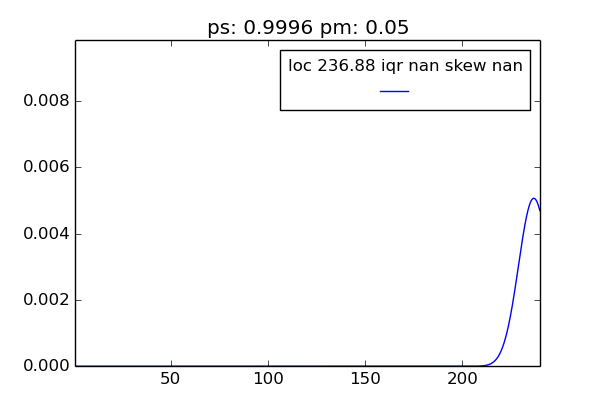
\includegraphics[width=0.49\textwidth]{bilder/outof240}
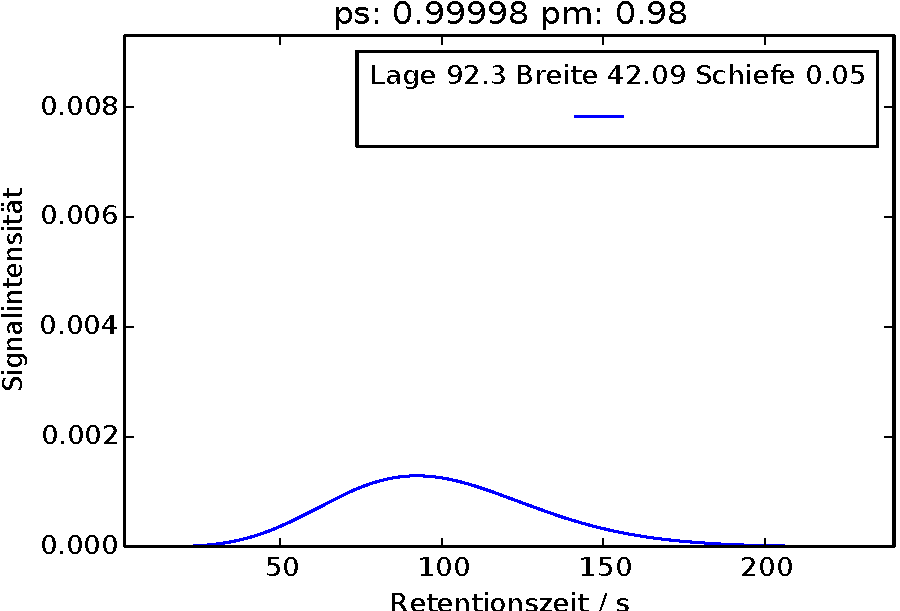
\includegraphics[width=0.49\textwidth]{bilder/huegel}
\caption[Nicht berücksichtigte Verteilungen]{Nicht berücksichtigte Verteilungen, links teilweise außerhalb des Chromatogramms, rechts zu breit}
\label{kein_peak}
\end{figure}

Auch von den übrigen, innerhalb des Zeitraumes von $240$ Sekunden liegenden Verteilungen, sind nicht alle als Peak zu bezeichnen. Beispielsweise kann eine Verteilung extrem breit sein und über das gesamte Spektrum reichen. Damit würde sie in einer echten Messung wohl eher als Hintergrundrauschen erkannt werden. Ein Beispiel dafür ist in rechts in Abbildung \ref{kein_peak} zu sehen. 
%Für die nachfolgenden Evaluationen wurde eine willkürliche Obergrenze bei einem IQR von $30$ gesetzt. Breitere Peaks können zwar mit den Modellen simuliert, werden aber nicht mehr berücksichtigt.

Für die Schiefe eines Peaks sollen keine Einschränkungen gemacht werden, es werden alle Werte im möglichen Intervall $[0,1]$ für den Quartilskoeffizienten untersucht werden. Um die Schiefe verschiedener Peaks besser einschätzen zu können, sind in Abbildung \ref{diverse_schiefen} Peaks mit verschieder Schiefe gezeigt.

\begin{figure}
 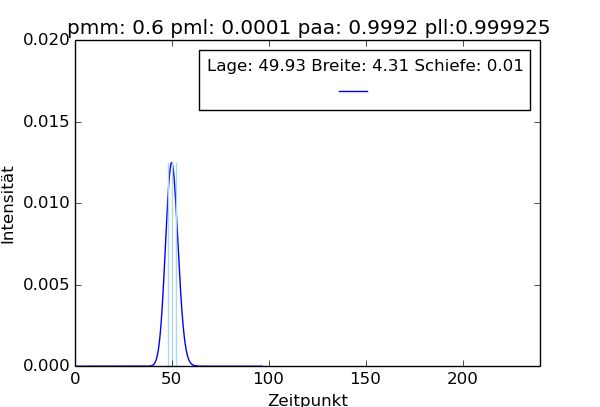
\includegraphics[width=0.49\textwidth]{bilder/Schiefe/001_q}
 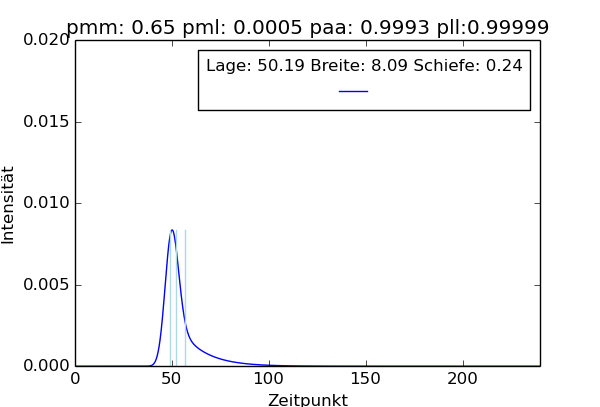
\includegraphics[width=0.49\textwidth]{bilder/Schiefe/025_q}
 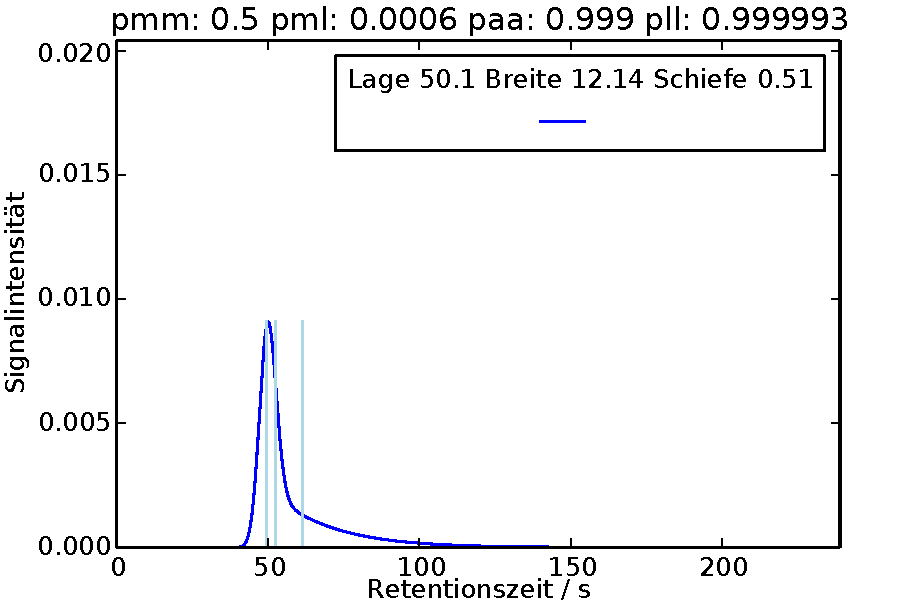
\includegraphics[width=0.49\textwidth]{bilder/Schiefe/05_q}
 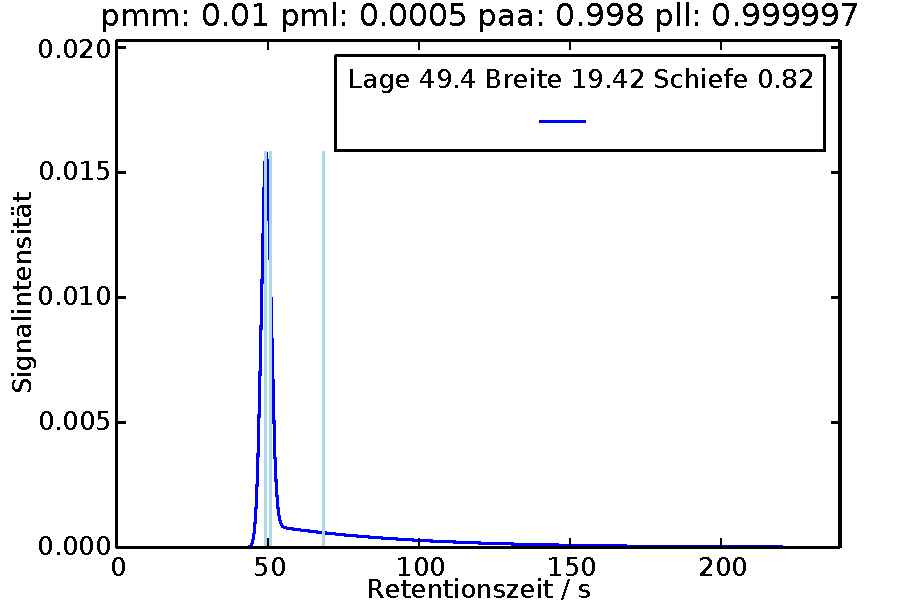
\includegraphics[width=0.49\textwidth]{bilder/Schiefe/08_q}
\caption{Peaks mit verschiedenen Schiefen}
\label{diverse_schiefen}
\end{figure}

Beim Peak unten rechts in Abbildung \ref{diverse_schiefen} mit der Schiefe von $0,82$ fällt auf, dass die Breite ebenfalls sehr groß ist, obwohl ein menschlicher Betrachter ihn wohl eher als schmaler als die anderen abgebildeten Peaks bezeichnen würde. Dies liegt an den verwendeten Maßen für Schiefe und Breite. Der Tail des Peaks hat zwar eine sehr niedrige Intensität im Vergleich zum Maximalwert, reicht jedoch über einen Großteil des restlichen Spektrums. Es kommt noch ein großer Teil der Teilchen deutlich nach dem Hauptpulk an, wodurch sich das $Q_{75}$ Quantil deutlich nach hinten verschiebt. Zur Verdeutlichung wurden die Quartile als senkrechte Linien mit in die Plots aufgenommen.

Wenn ein solcher Peak in einer tatsächlichen Messung vorkäme, könnte es gut sein, dass der Tail auf Grund seiner niedrigen Intensität jedoch gar nicht mehr als zum Peak gehörig erkannt würde, sonder eher dem Hintergrundrauschen zugerechnet würde. \todo{Diskussion: Andere Maße testen}

%Wo genau eine sinnvolle Obergrenze für die Breite der Peaks liegt, ist schwer abzugrenzen, dazu wäre eine ausführliche Auswertung  


\section{2-Zustände Modell} 
Zunächst wird der Einfluss der beiden Parameter auf die Peaks beschrieben. Da sich die Intensität dieses Einflusses je nach Wert des anderen Parameters verändert, wird anschließend der gemeinsame Einfluss der beiden Parameter betrachtet. Außerdem wird beschieben, was nicht mit dem Modell simuliert werden kann.

\subsection{Einfluss der Parameter auf einzelne Peaks}

% \begin{figure}[h]
% \centering
% \caption{Peak zum Zeitpunkt $t \approx 20$}
% \label{2s_t20}
% \end{figure}
Es wird an zwei einzelnen Peaks gezeigt, wie sich die Veränderung von jeweils einem Parameter auf die Peakcharakteristika auswirkt. Beide dieser Peaks könnten so ein einem echten Chromatogramm beobachtet worden sein.

\begin{figure}[H]
\begin{center}
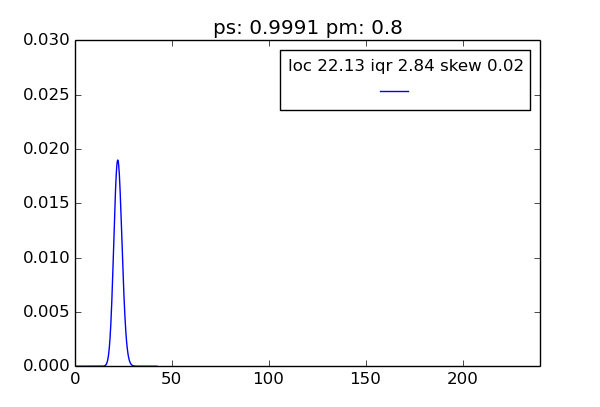
\includegraphics[width=0.49\textwidth]{bilder/2s_t20}
\end{center}
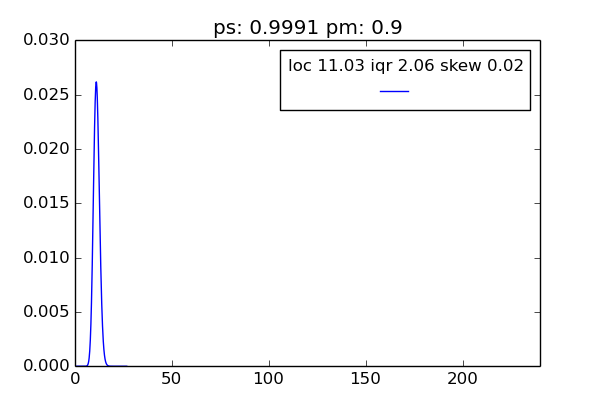
\includegraphics[width=0.49\textwidth]{bilder/2s_t20_pmp}
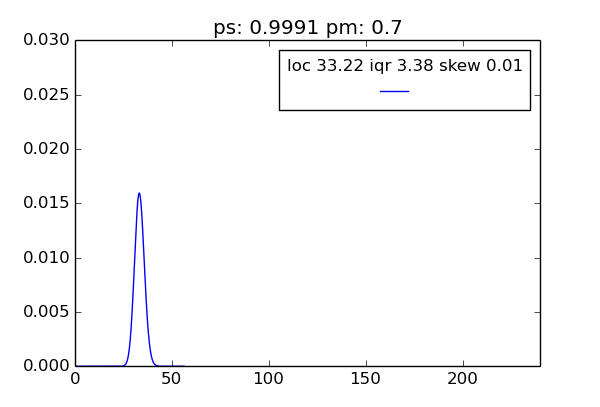
\includegraphics[width=0.49\textwidth]{bilder/2s_t20_pmm}
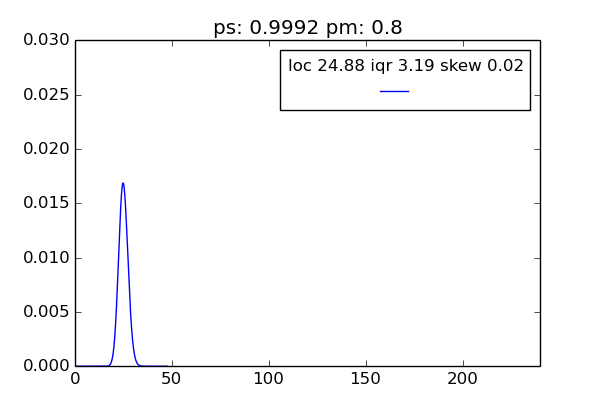
\includegraphics[width=0.49\textwidth]{bilder/2s_t20_psp}
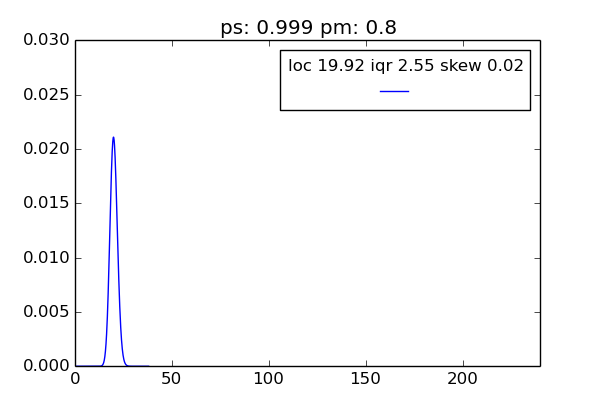
\includegraphics[width=0.49\textwidth]{bilder/2s_t20_psm}
\caption[Einfluss von pm und ps auf einen Peak]{Einfluss von pm und ps auf einen Peak, oben der Ausgangspeak mit $pm = 0,8$ und $ps = 0,9991$, veränderte Parameter: in der Mitte links $pm = 0,9$, rechts $pm = 0,7$, unten links $ps = 0,999$, rechts $ps = 0,9992$ }
\label{2s_t20_change}
\end{figure}

In Abbildung \ref{2s_t20_change} ist ein Peak zu sehen, der mit den Parametern $pm = 0,8$ und $ps = 0,9991$ simuliert wurde. Sein Maximalwert liegt bei etwa $t = 22$ s und er hat eine Breite von etwa $2,8$. Abbildung \ref{2s_t100_change} zeigt einen Peak, dessen Maximalwert bei $t=100$ s liegt und der einen Interquartilsabstand von $7,4$ hat. Er wurde mit den Parametern $pm = 0,5$ und $ps = 0,9995$ simuliert.
\begin{figure}[h]
\begin{center}
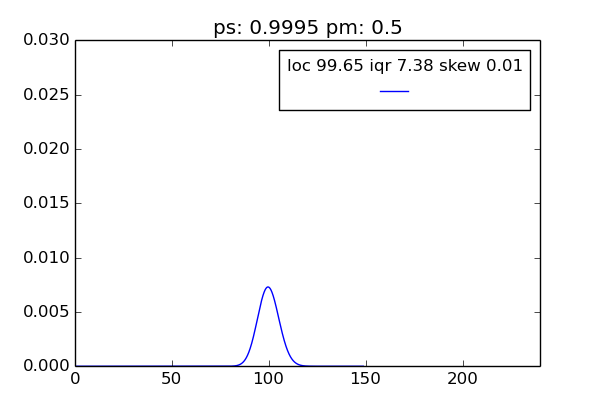
\includegraphics[width=0.49\textwidth]{bilder/2s_t100}
\end{center}
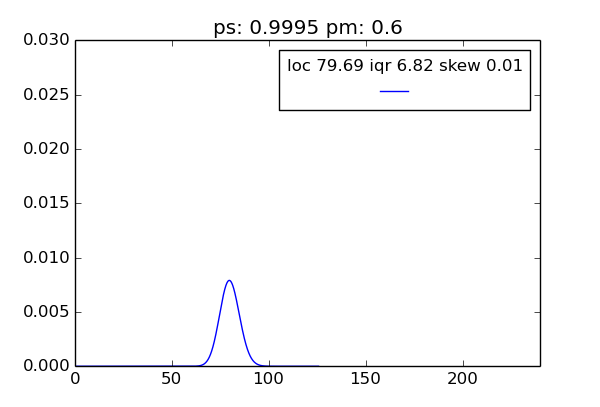
\includegraphics[width=0.49\textwidth]{bilder/2s_t100_pmp}
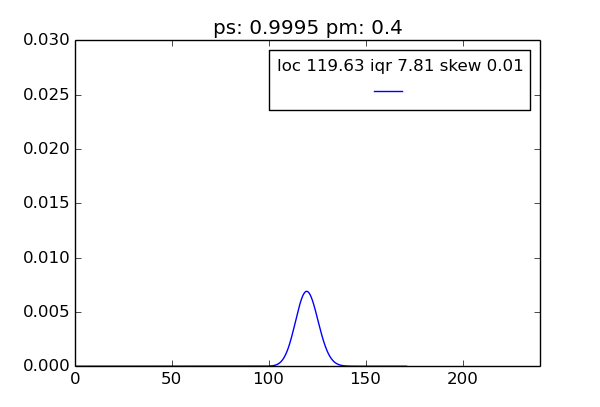
\includegraphics[width=0.49\textwidth]{bilder/2s_t100_pmm}
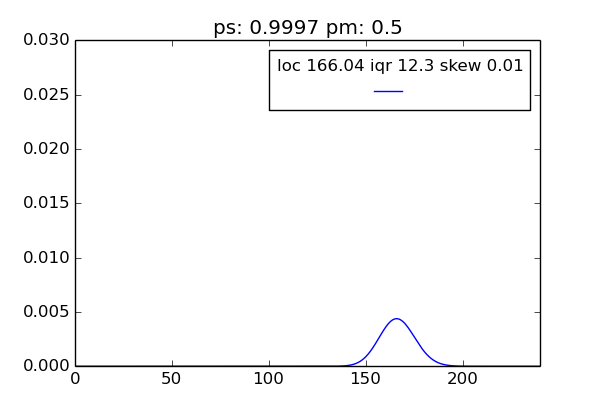
\includegraphics[width=0.49\textwidth]{bilder/2s_t100_psp}
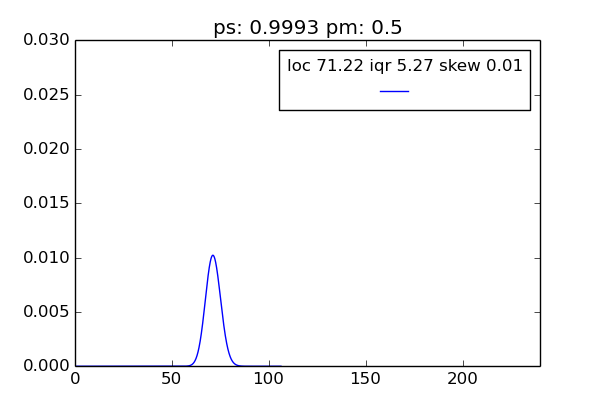
\includegraphics[width=0.49\textwidth]{bilder/2s_t100_psm}
\caption[Einfluss von pm und ps auf einen Peak]{Einfluss von pm und ps auf einen Peak, oben der Ausgangspeak mit $pm = 0,5$ und $ps = 0,9995$, veränderte Parameter: in der Mitte links $pm = 0,6$, rechts $pm = 0,4$, unten links $ps = 0,9993$, rechts $ps = 0,9997$ }
\label{2s_t100_change}
\end{figure}

In beiden Fällen zeigen sich bei Veränderungen an den Parametern die gleichen Effekte am Peak. Wenn pm größer oder ps kleiner wird, resultiert ein schmalerer und früherer Peak. Umgekehrt bewirkt eine Verkleinerung von pm oder eine Vergrößerung von ps, einen späteren und breiteren Peak. Die Schiefe verändert sich, wenn überhaupt, nur minimal.
Die Stärke der Veränderung an den Peaks unterscheidet sich jedoch in beiden Fällen. Daher wird im nächsten Abschnitt untersucht, inwiefern der Einfluss eines Parameters größer oder kleiner wird, abhängig davon, welchen Wert der andere Parameter annimmt.

\subsection{Einfluss abhängig vom anderen Parameter}

Um den Einfluss der Parameter in Abhängigkeit vom anderen Parameter zu untersuchen, werden im Folgenden Plots verwendet, bei denen ein Parameter fest ist, der andere jedoch verschiedene Werte annimmt. Alle Plots wurden mit der gleichen Achseneinteilung gemacht, um eine bessere Vergleichbarkeit zu ermöglichen. Jeder Peak wird dargestellt durch einen Punkt an den Koordinaten seines Zeitpunktes und seiner Schiefe. Die Größe des Punktes wird festgelegt durch die Breite des entsprechenden Peaks. Zusätzlich ist die Breite in der Legende noch einmal aufgeführt. Beschriftet ist jeder Punkt mit dem variablen Parameter des Vergleichsplots, in der Überschrift ist jeweils der Wert des festen Parameters zu finden.


\begin{figure}[h]
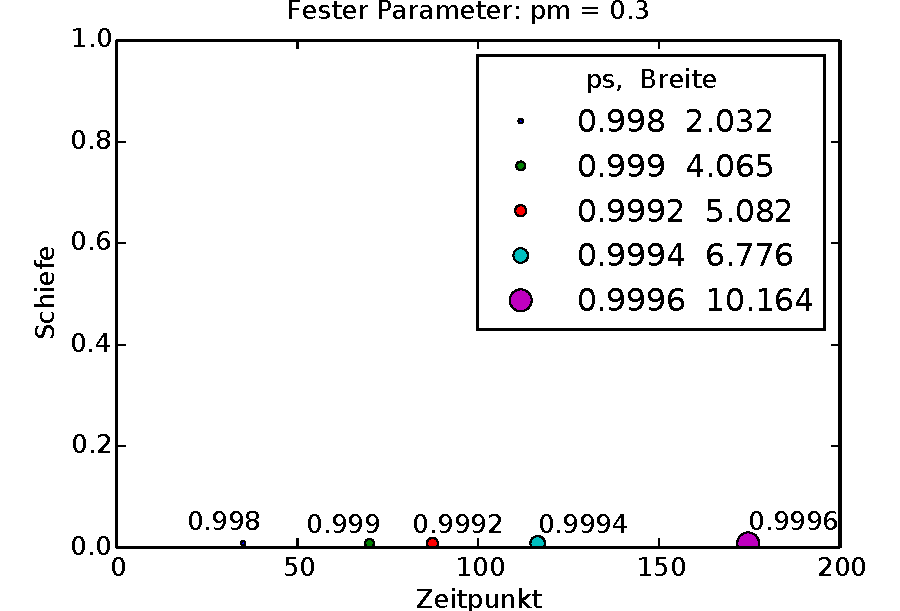
\includegraphics[width=0.49\textwidth]{bilder/ps/psfest_pm03}
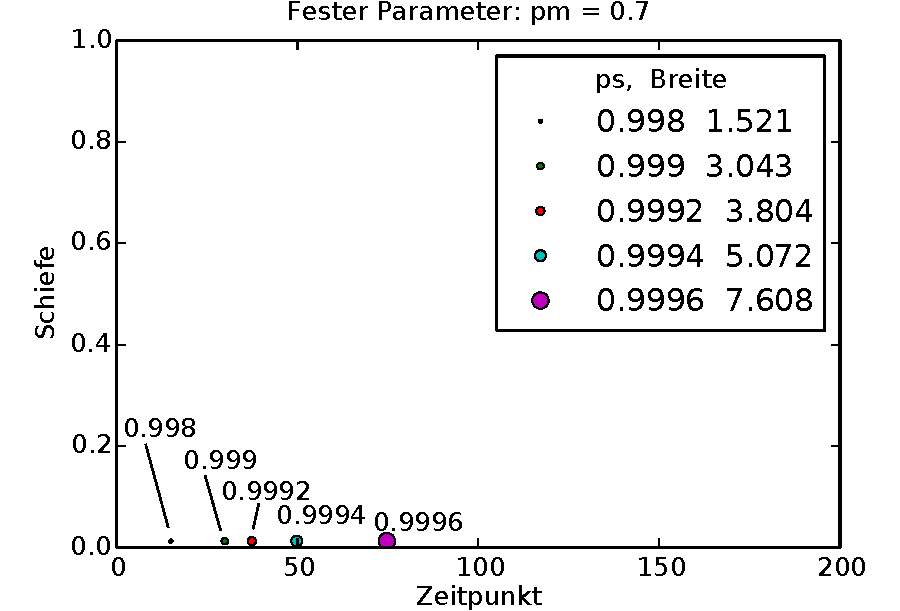
\includegraphics[width=0.49\textwidth]{bilder/ps/psfest_pm07}
\caption{Der Einfluss von $p_{s}$ auf die Peaks abhängig von $p_{m}$}
\label{einfluss_ps_1}
\end{figure}

In Abbildung \ref{einfluss_ps_1} ist der Einfluss des Parameters ps in Abhängigkeit von pm gezeigt. Neben der bereits im letzten Abschnitt gewonnenen Erkenntnis, dass die Peaks mit zunehmendem ps breiter werden und später erscheinen, ist zu sehen, dass der Einfluss von ps größer wird, wenn pm kleiner ist. Dies gilt sowohl für den Zeitpunkt, als auch die Breite des Peaks. Die Schiefe wird in beiden Fällen nicht wahrnehmbar beeinflusst.

\begin{figure}[h]
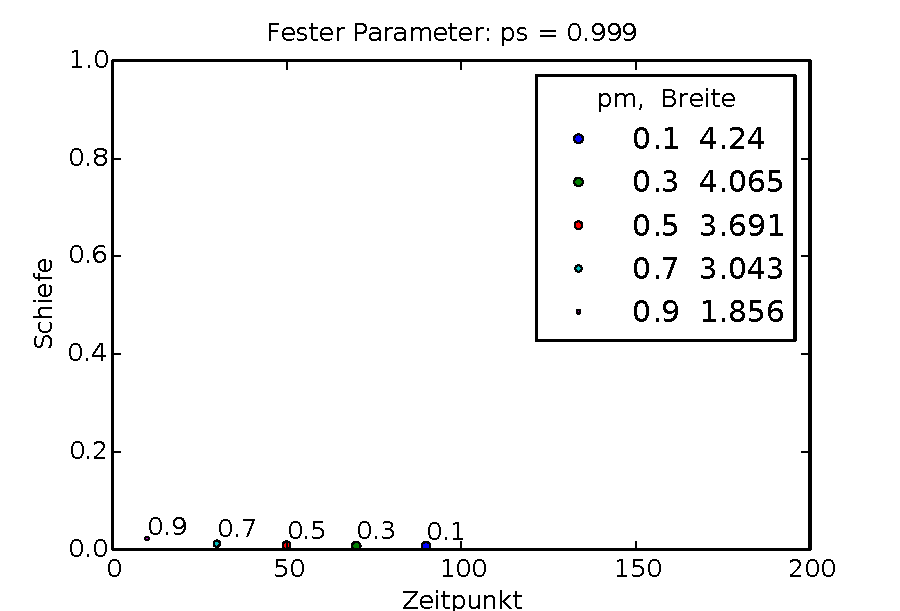
\includegraphics[width=0.49\textwidth]{bilder/pm/pmfest_ps0999}
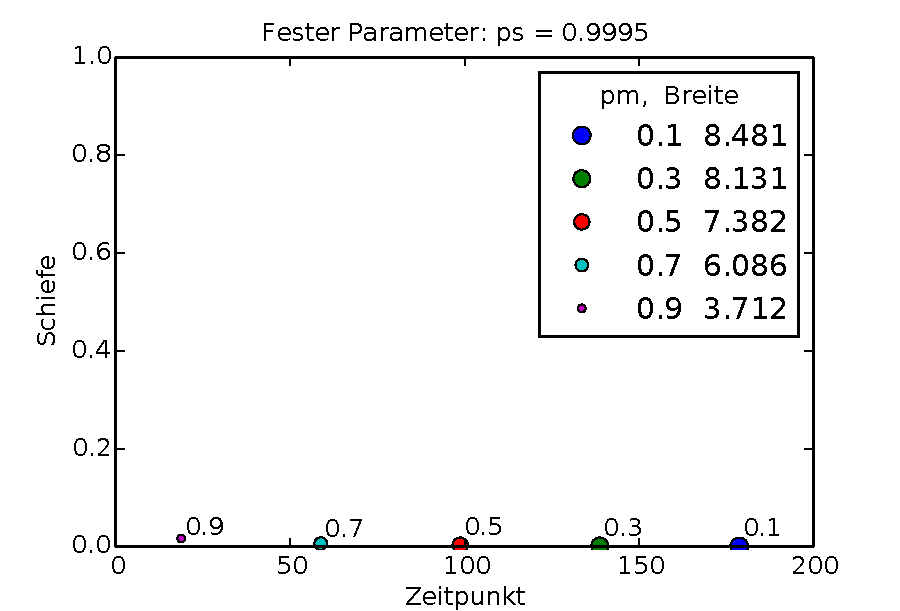
\includegraphics[width=0.49\textwidth]{bilder/pm/pmfest_ps09995}
\caption{Der Einfluss von $p_{m}$ auf die Peaks abhängig von $p_{s}$}
\label{einfluss_pm_1}
\end{figure}

Der Einfluss des Parameters pm in Abhängigkeit von ps ist in Abbildung \ref{einfluss_pm_1} zu dargestellt. Auch hier ist der Einfluss von pm auf Breite und Lage der Peaks erkennbar, der stärker ist bei größerem ps. Zu erkennen ist hier auch eine geringe Zunahme der Schiefe mit steigendem pm. Diese Veränderung ist jedoch nicht abhängig von ps.

%Schiefe nur von pmm beeinflusst. Auch wenn pm auf den Wert von 0.999 gesetzt ist, was ja schiefe verursacht, ergeben alle ps's gleiche schiefe. Umgekehrt erzeugen bei festem ps jeweils die pm von ca 0.999 schiefe peaks bei sehr kleinen zeitpunkten (loc = 0.1, also minimalzeitpunkt) Das sieht so aus, als würde der direkt am beginn starten, aber das ist der kompression geschuldet, wenn ich nur ein zehntel komprimiere, hat der peak vorlauf

\section{Grenzen}
Mit diesem Modell sind kaum tailende Peaks erzeugbar. Schiefe von mehr als $0,05$ tritt nur selten auf, immer bei Peaks, die ihren Maximalzeitpunkt ganz am Anfang des Spektrums, knapp über der Trägergaszeit von $0,1$ Sekunden haben. Der Effekt wird verursacht durch einen sehr großen Wert für pm, der bei ungefähr $0,999$ liegt. Dadurch gibt es viele Teilchen die (bei einer Säulenlänge von $1000$ Schritten) gar nicht in Wechselwirkung mit der stationären Phase geraten und dadurch mit Trägergasgeschwindigkeit durch die Säule wandern. Die wenigen Teilchen, die doch in die stationäre Phase eintreten, verursachen den Tail, da sie deutlich später als der Pulk die Säule verlassen.

Eine weitere Grenze ist jedoch die Minimalbreite der erzeugten Peaks. Damit ist gemeint, dass mit zunehmender Zeit die Minimalbreite der Peaks, die an diesem Zeitpunkt ihr Maximum haben, ansteigt. Zur Verdeutlichung ist in Abbildung \ref{Grenzen_2p_ohnep} eine Übersicht über die erreichbaren Zeit-Breiten Kombinationen gegeben. Jeder Punkt steht für einen Peak, der mit der entsprechenden Maximalzeit und Breite erzeugt wurde.
Zu sehen ist, dass es zu jedem Zeitpunkt möglich ist, Peaks mit dem Modell zu erzeugen. Auch zwischen den einzelnen Punkten sind Peaks erzeugbar, wenn die Parameter entsprechend angepasst werden.

\begin{figure}[h]
\centering
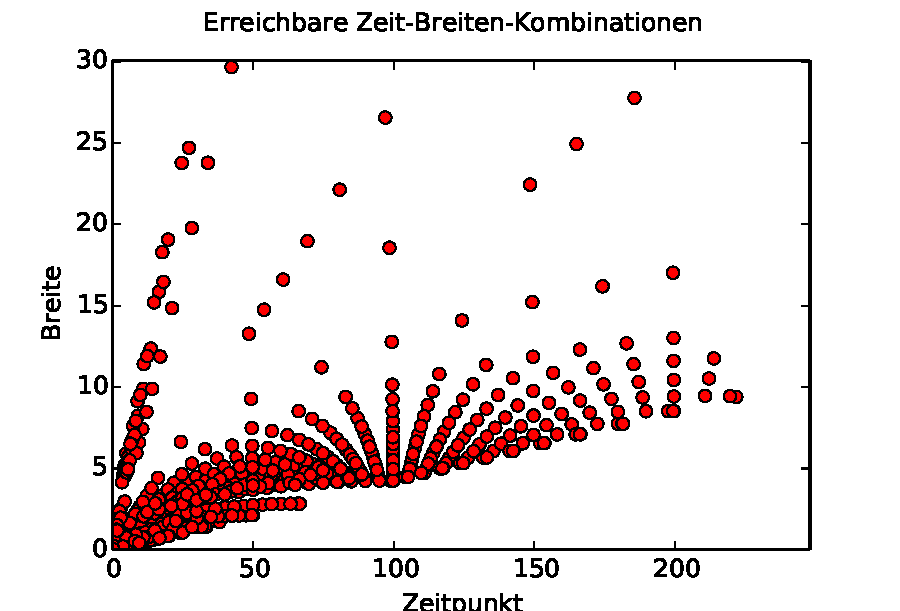
\includegraphics[width=0.75\textwidth]{bilder/2s_zeitbreiten_ohnep}
\caption{Mit dem 2-Zustände Modell erreichbare Zeitpunkte und Breiten}
\label{Grenzen_2p_ohnep}
\end{figure}

Dass die untere Kante der Punktewolke jedoch eine Grenze für die Breite darstellt, ist in Abbildung \ref{Grenzen_2p_ausschnitt} zu sehen. Zu sehen sind zwei Reihen von Peaks, die mit jeweils dem gleichen Parameter ps erzeugt wurden, die Breite nimmt mit fallendem pm zu. Diese Beobachtung wurde bereits im letzten Abschnitt gemacht. Jedoch ist hier zu sehen, dass sich bei einer Annäherung von pm an $0$ keine deutlich späteren Peaks ergeben, sondern der Zeitpunkt auf einem Wert stagniert. Das liegt daran, dass bei so kleinen Werten für pm in fast jedem Schritt, der in der mobilen Phase startet, ein Wechsel zur stationären Phase statt findet. Der Zeitpunkt wird dann also maßgeblich durch ps beeinflusst. Da höhere Werte für ps nicht nur für einen späteren Zeitpunkt sorgen, sondern auch für eine größere Breite, ergibt sich dadurch eine Minimalbreite für alle Zeitpunkte.

\begin{figure}[h]
\centering
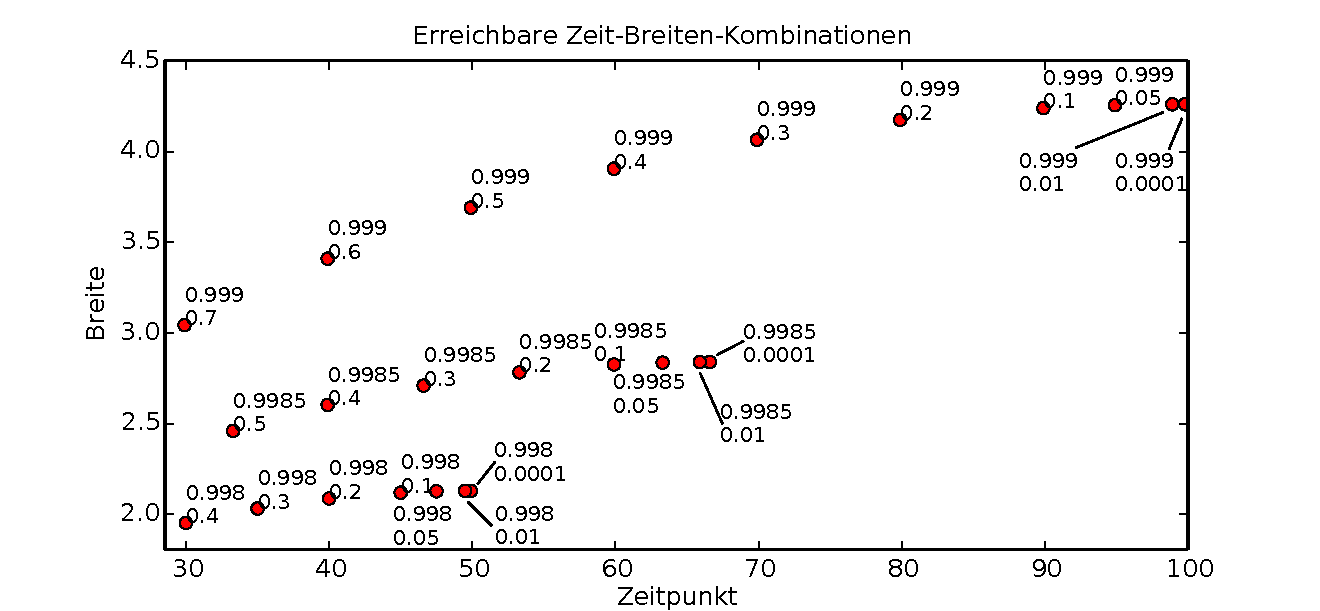
\includegraphics[width=0.75\textwidth]{bilder/2s_zeitbreiten_ausschnitt.pdf}
\caption{Ausschnitt der erreichbaren Zeiten und Breiten}
\label{Grenzen_2p_ausschnitt}
\end{figure}

Auch die obere Kante der Punktewolke aus Abbildung \ref{Grenzen_2p_ohnep} stellt gewissermaßen eine Grenze für die mit diesem Modell erreichbaren Zeit-Breiten Kombinationen dar. Zwar können in dem Bereich, der Tailing aufweist, fast beliebig breite Peaks erzeugt werden, wenn ps sehr groß gewählt wird. \todo{obergrenze?}


\section{3-Zustände Modell}
Die wenigen Peaks, die beim 2-Zustände Modell Schiefe aufweisen dienen als Hinweis darauf, wie das Tailing entsteht: Einige wenige Teilchen kommen deutlich nach dem Hauptpulk an, da sie in der stationären Phase verweilen, während die Teilchen des Pulks ohne Interaktion die Säule durchqueren. 
Wenn nun bei einer beliebigen, nicht-tailenden Verteilung, die dadurch entsteht, dass immer wieder Teilchen mit der stationären Phase interagieren, ein zusätzlicher Zustand hinzugefügt wird, in den die Teilchen seltener, aber dafür viel länger eintreten, müsste genau dieser Effekt auch bei anderen als den ganz frühen Verteilungen entstehen.

Genau dieser Zustand steht im 3-Zustände Modell zur Verfügung. Untersucht wurde vor allem das Modell aus Abbildung \ref{tikz:4p_Mod_a}, bei dem die beiden stationären Zustände getrennt sind.

Im Folgenden werden die Einflüsse der Parameter dieses Modells untersucht, dabei beschränkt sich diese Untersuchung auf pmm, pml, paa und pll. Die anderen Parameter pma, pam und plm können daraus berechnet werden.


% \subsection{Relevanter Parameterbereich / relevante Peaks}
% Die wenigen Peaks, die beim 2-Zustände Modell Schiefe aufweisen dienen als Grundlage für eine sinnvolle Parametereinschränkung für $p_{ml}$ und $p_{ll}$. Dabei war zu beobachten, dass Tailing nur dann auftritt, wenn die Teilchen nur selten in den stationären Zustand eintreten, dafür aber sehr lange dort verweilen. Um diesen Effekt nachzuahmen, muss $p_{ml}$ dementsprechend sehr klein im Vergleich zu $p_{ma}$ und $p_{mm}$ sein, außerdem muss $p_{ll}$ sehr groß sein, deutlich größer als $p_{aa}$.
% 
% In der experimentellen Phase der Arbeit wurden zunächst im gesamten Parameterraum %$[0;1]^3$ 
% einige Simulationen durchgeführt, um herauszufinden, in welchen Bereichen sich Verteilung ergeben, die als Peaks interpretiert werden können. 
% Durch die Beschränkung des Spektrums auf $240$ Sekunden scheiden schon viele Parameterkombinationen aus, welche spätere Peaks erzeugen würden. Das betrifft insbesondere diejenigen Kombinationen, die eine geringe Wahrscheinlichkeit haben, mobil zu bleiben oder zu werden, dafür aber mit einer sehr hohen Wahrscheinlichkeit stationär werden oder bleiben. 
% % Für die Schiefe soll es zunächst keine Beschränkungen geben, TODO (gibt es ne sinnvolle Obergrenze, Optik mit Werten vergleichen)
% Typischerweise sind Peaks zu Beginn des Spektrums eher schmal, spätere Peaks können breiter werden. 
% Generell lässt sich sagen, dass der IQR eines Peaks geringer sein sollte, als sein Maximalzeitpunkt, ansonsten ist er schwer als Peak zu identifzieren. Darüber hinaus wurde eine maximale Peakbreite von TODO $10+0.2\cdot t_{max}$ \todo{sinnvolle maximalbreite} festgelegt. Peaks mit höherem IQR sind in einem Spektrum kaum noch als Peaks zu erkennen.
% Durch die Verwendung von IQR und IKQ als Maße für Breite und Schiefe, sind sehr breite Peaks auch dann als Peak zu erkennen, wenn sie sehr schief sind.
% 
% Für die Schiefe gilt, dass ein Tailing ab einem IQK von 0.2 gut zu erkennen ist. Werte bis 0.4 treten meist bei schiefen Peaks auf, die auch vom optischen Eindruck einem realistischen Peak ähneln. Werte darüber hinaus deuten meist auf ein sehr langes Tailing, welches teilweise auch über die Maximalzeit hinausragt. Dieses Tailing ist jedoch auf einem so niedrigen Niveau, dass es in einer realen Messung wahrscheinlin im Rauschen unter gehen würde.
% 
% Dadurch ergeben sich folgende Einschränkungen für die verschiedenen Parameter:
% \begin{itemize}
%  \item $p_{mm}$: keine generellen Einschränkungen, es wurden für Werte im Intervall $[0,005; 0,99]$ Peaks gefunden. Bei noch kleineren Werten und auch bei Werten im unteren Bereich des Intervalls kommen abhängig von den anderen Parametern zu späte Peaks heraus. Bei größeren Werten dominiert dieser Parameter zu sehr, sodass nur extrem frühe und schmale sowie kaum schiefe Peaks entstehen.
%  \item $p_{ml}$: sinnvolle Werte liegen im Bereich $[0,00005; 0,005]$. Bei kleineren Werten ergeben sich auch Peaks, welche jedoch kein oder fast kein Tailing mehr aufweisen, sodass auch auf das 2-Zustände Modell zurückgegriffen werden kann. Bei größeren Werten verweilen die Teilchen so häufig im gelösten Zustand, dass die Peaks extrem breit werden. Insbesondere, wenn der Parameter $p_{ll}$ auch sehr groß gewählt wurde, gilt dies auch für hohe Werte für $p_{ml}$ innerhalb des Intervalls.
%  \item $p_{aa}$: für diesen Parameter wurde das Intervall auf $[0,997; 0,9996]$ beschränkt. Kleinere Werte sorgen für extrem frühe Peaks. Diese könnten zwar berücksichtigt werden, unterscheiden sich jedoch kaum voneinander. Bei größeren Werten werden die Peaks meist sehr breit oder ragen über die Maximalzeit hinaus. 
%  \item $p_{ll}$: sinnvolle Werte liegen im Bereich $[0,9999; 0,999995]$. Bei Werten ab dem unteren Intervallbereich ergeben keine oder nur kaum schiefe Peaks. Bei größeren Werten werden die Teilchen so lange im stationären Zustand gehalten, dass das Tailing meist weit über das Maximum von 240 Sekunden hinausragt oder Peaks zu breit werden. Dies gilt insbesondere, wenn für $p_{ml}$ ebenfalls ein großer Wert gewählt wurde. 
%  %Im oberen Bereich des Intervalls (>0.999995) erzeugen werden hier Peaks erzeugt, die eine sehr große Schiefe aufweisen, wo der Tail jedoch (wahrscheinlich) im Rauschen verschwindet. Mit den aktuellen Maßen lässt sich das kaum zeigen, wird jedoch beim Blick auf einen geplotteten Peak sofort klar.
% \end{itemize}
% 
% In allen Fällen gilt jedoch, dass auch jeweils die Kombination der Parameter berücksichtigt werden muss, insbesondere, wenn ein Parameter am Rand des jeweils angegebenen Intervalls liegt, kommt es häufig vor, dass er nur in einigen wenigen Kombinationen für realistische Peaks sorgt.
% \todo{Beispiele; ein paar Kombis nennen, die grenzwertig, bzw drüber hinaus sind?}


% \subsection{Einfluss der verschiedenen Parameter auf Peaks}
% Auch bei 3 Zuständen können in den meisten Fällen ein deutlicher Zusammenhang zwischen den Parametern und Peakdaten beobachtet werden, diese seien im Folgenden aufgeführt.

\subsection{Einfluss auf einzelne Peaks}
Um den Einfluss der Parameter auf Peaks zu untersuchen, wurden zunächst einige realistische Ausgangspeaks gewählt. Die dafür verwendeten Simulationsparameter wurden dann nur wenig verändert und beobachtet, wie sich der Peak verändert. In \ref{einfluss_t50} und \ref{einfluss_t100} ist jeweils gezeigt, wie der Peak auf die Veränderungen reagiert. 

Zu erkennen ist, dass eine Veränderung von pmm und paa jeweils die Lage des Peaks beeinflusst, hingegen eine Änderung von pml oder pll kaum einen Einfluss auf die Lage hat. Umgekehrt wird die Breite hauptsächlich durch pml und pll verändert, jedoch nur minimal von pmm und paa. 


\begin{table}[]
\centering
\caption{Einfluss auf einen Peak (1)}
\label{einfluss_t50}
\begin{tabular}{|l|l|l|l||l|l|l|}
\hline
pmm & pml    & paa    & pll      & Lage  & Breite & Schiefe \\ \hline \hline
$$0,6$$ & $0,0006$ & $0,9992$ & $0,999993$ & $50,14$ & $12,34$  & $0,46$    \\ \hline \hline
\cellcolor{yellow} $0,5$ & $0,0006$ & $0,9992$ & $0,999993$ & $62,69$ & $12,45$  & $0,43$    \\ \hline
\cellcolor{yellow} $0,7$ & $0,0006$ & $0,9992$ & $0,999993$ & $37,59$ & $12,2$   & $0,5$     \\ \hline
$0,6$ & \cellcolor{yellow} $0,0005$ & $0,9992$ & $0,999993$ & $50,09$ & $9,7$    & $0,38$    \\ \hline
$0,6$ & \cellcolor{yellow} $0,0007$ & $0,9992$ & $0,999993$ & $50,19$ & $14,82$  & $0,5$     \\ \hline
$0,6$ & $0,0006$ & \cellcolor{yellow} $0,9991$ & $0,999993$ & $44,55$ & $12,18$  & $0,5$     \\ \hline
$0,6$ & $0,0006$ & \cellcolor{yellow} $0,9993$ & $0,999993$ & $57,33$ & $12,57$  & $0,41$    \\ \hline
$0,6$ & $0,0006$ & $0,9992$ & \cellcolor{yellow} $0,99999$  & $50,25$ & $9,2$    & $0,33$    \\ \hline
$0,6$ & $0,0006$ & $0,9992$ & \cellcolor{yellow} $0,999995$ & $50,05$ & $16,66$  & $0,58$    \\ \hline
\end{tabular}
\end{table}


\begin{table}[]
\centering
\caption{Einfluss auf einen Peak (2)}
\label{einfluss_t100}
\begin{tabular}{|l|l|l|l||l|l|l|}
\hline
pmm & pml    & paa    & pll      & Lage  & Breite & Schiefe \\ \hline \hline
 $0,1$ & $0,0005$  & $0.9991$  & $0.99999$  & $100,22$  & $8,1$  & $0,23$ \\ \hline
 $0,05$ & $0,0005$  & $0.9991$  & $0.99999$  & $105,76$  & $8,11$  & $0,23$ \\ \hline
 $0,2$ & $0,0003$  & $0.9991$  & $0.99999$  & $89,1$  & $8,05$  & $0,23$ \\ \hline
 $0,1$ & $0,0007$  & $0.9991$  & $0.99999$  & $100,04$  & $6,22$  & $0,12$ \\ \hline
 $0,1$ & $0,0005$  & $0.9991$  & $0.99999$  & $100,4$  & $10,89$  & $0,34$ \\ \hline
 $0,1$ & $0,0005$  & $0.999$  & $0.99999$  & $90,17$  & $7,68$  & $0,26$ \\ \hline
 $0,1$ & $0,0005$  & $0.9992$  & $0.99999$  & $112,77$  & $8,64$  & $0,2$ \\ \hline
 $0,1$ & $0,0005$  & $0.9991$  & $0.999975$  & $100,41$  & $5,91$  & $0,8$ \\ \hline
 $0,1$ & $0,0005$  & $0.9991$  & $0.999993$  & $100,12$  & $9,93$  & $0,34$ \\ \hline
\end{tabular}
\end{table}


\subsubsection{Einfluss abhängig von anderen Parametern}

%\subsection{3-Zustände Modell}
Bei diesem Modell ergeben sich durch die größere Anzahl an Parametern, komplexere Zusammenhänge zwischen den Parametern und den Peakdaten. Teilweise hängt die Stärke des Einflusses eines Parameters auf ein Peakcharakteristikum vom Wert eines anderen Parameters ab. Das heißt, der Einfluss eines Parameters auf die resultierenden Peaks kann größer oder kleiner sein, abhängig davon, ob ein anderer Parameter eher im oberen oder unteren Bereich seines oben angegebenen Intervalls liegt.
Zunächst können jedoch folgenden einfachen Zusammenhänge beobachtet werden:

Für den Maximalzeitpunkt des Peaks sowie seine Breite gilt, dass beide größer werden, wenn die Parameter $p_{ml}$, $p_{aa}$ und $p_{ll}$ größer werden oder $p_{mm}$ kleiner wird. 
Die Schiefe steigt mit fallendem $p_{aa}$ und in den meisten Fällen mit steigendem $p_{mm}$. Für $p_{ml}$, $p_{ll}$ und in wenigen Fällen auch $p_{mm}$ ist zu beobachten, dass bei größer werdenden Parametern die Schiefe zunächst auch ansteigt, ab einem gewissen Wert jedoch sinkt.

Insgesamt gilt, dass die Einflüsse auf Zeitpunkt und Breite der Peaks weniger komplex sind, als die Einflüsse auf die Schiefe. Das ist auch damit erklärbar, dass für Zeitpunkt und Breite eigentlich nur die zwei Parameter des einfachen Modells nötig sind und die Aufsplittung des stationären Zustands daran nicht viel ändert. Die Schiefe jedoch hängt immer von mehreren Parametern und deren Kombination ab.

Im Folgenden ist für jeden der vier Parameter eine detaillierte Übersicht gegeben welche Eigenschaften der Peaks er in Abhängigkeit anderer Parameter beeinflusst. Die zur Verdeutlichung verwendeten Plots sind denen aus der Auswertung des 2-Zustände Modells sehr ähnlich, hier wurden drei der vier Parameter fest gehalten, der vierte wird variiert. Auch diese Plots wurden zur besseren Vergleichbarkeit weiterhin mit der gleichen Achseneinteilung erstellt. 

\todo{Plotbeschriftung (Titel), Plots nachbearbeiten, Achenbeschrifung und überschrift größer}

\paragraph*{Einfluss des Parameters $p_{mm}$}

% \begin{figure}
% \begin{subfigure}{0.6\textwidth}
% 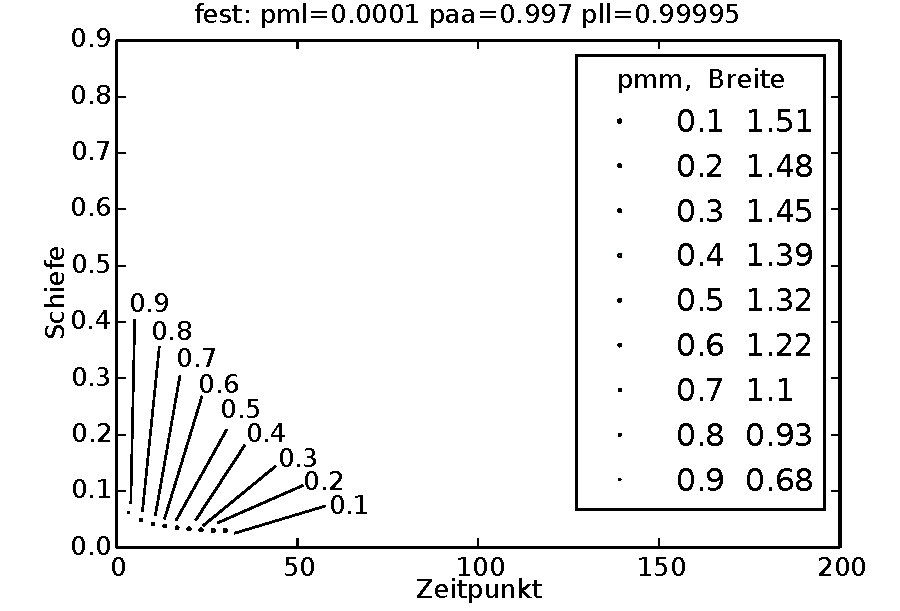
\includegraphics[width=\textwidth]{bilder/pmm/3fest_p_00001_0997_099995}
% \caption{$p_{aa}$ klein}
% \end{subfigure}
% 
% \begin{subfigure}{0.6\textwidth}
% 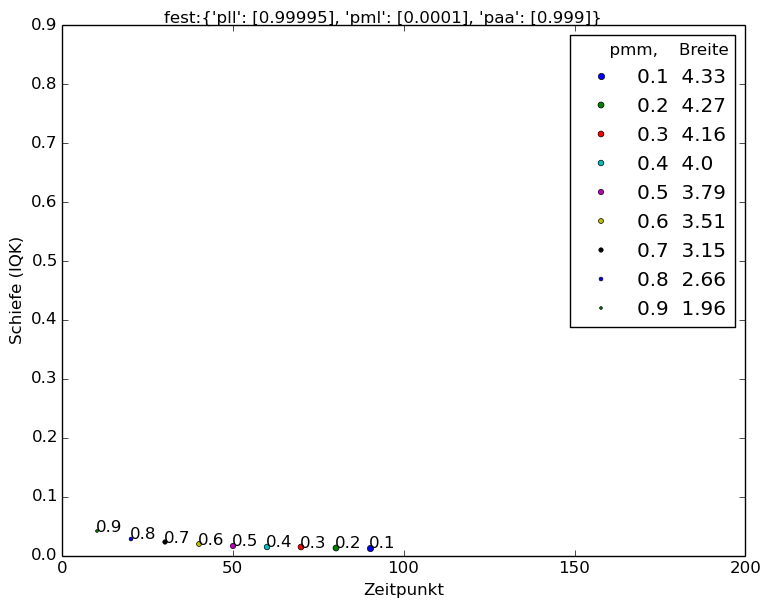
\includegraphics[width=\textwidth]{bilder/pmm/3fest_p_00001_0999_099995}
% \caption{$p_{aa}$ mittel}
% \end{subfigure}
% 
% \begin{subfigure}{0.6\textwidth}
% 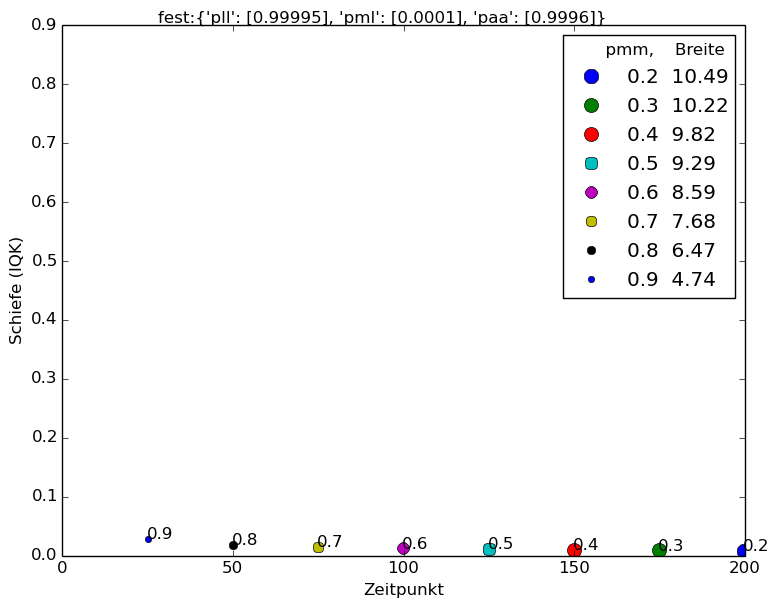
\includegraphics[width=\textwidth]{bilder/pmm/3fest_p_00001_09996_099995}
% \caption{$p_{aa}$ groß}
% \end{subfigure}
% \caption{Der Einfluss von $p_{mm}$ auf die Peaks abhängig von $p_{aa}$}
% \label{einfluss_pmm_1}
% \end{figure}

\begin{figure}[h]
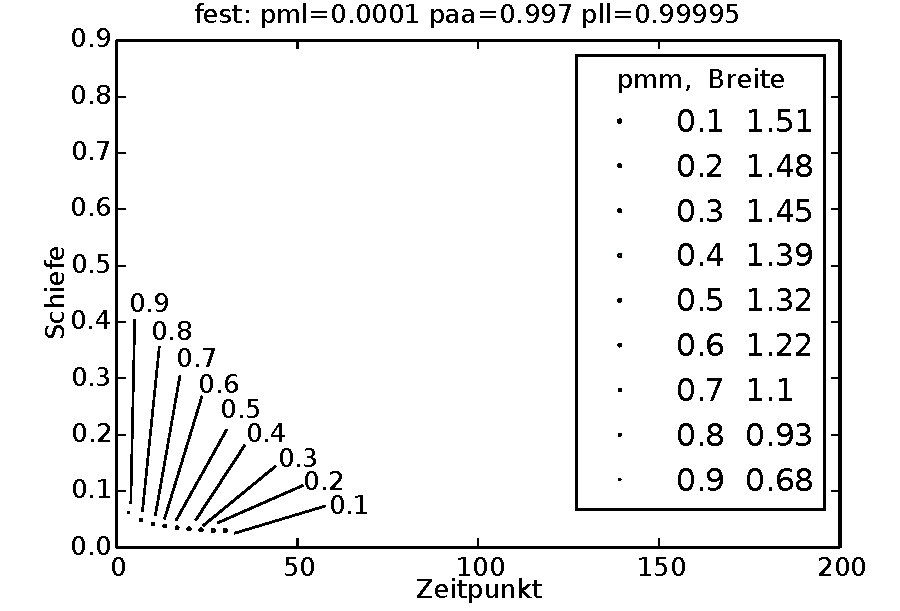
\includegraphics[width=0.49\textwidth]{bilder/pmm/3fest_p_00001_0997_099995}
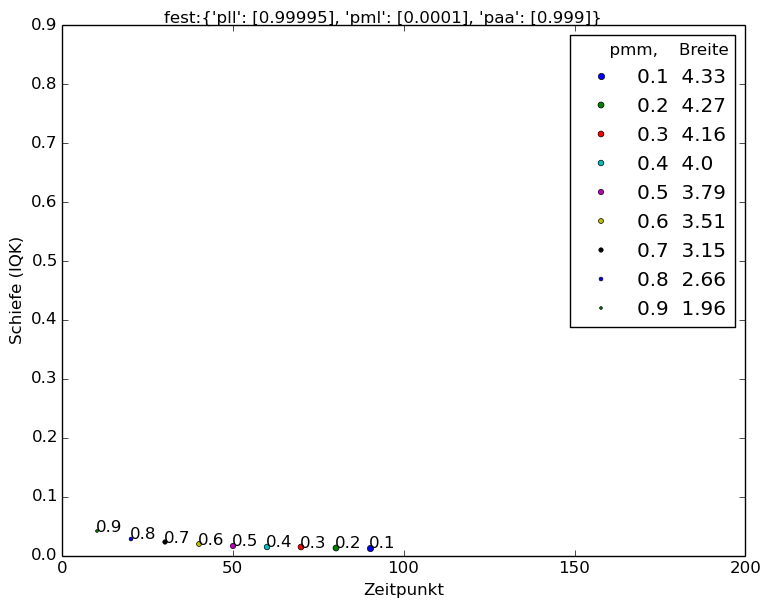
\includegraphics[width=0.49\textwidth]{bilder/pmm/3fest_p_00001_0999_099995}

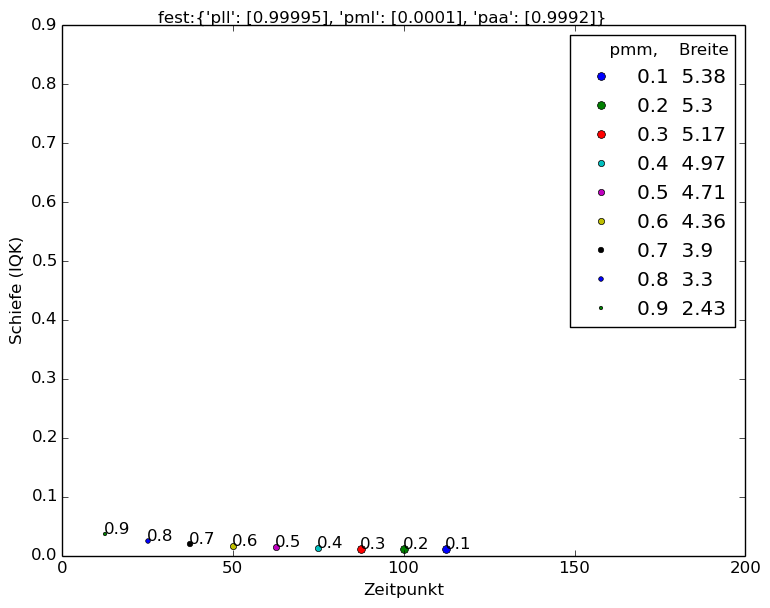
\includegraphics[width=0.49\textwidth]{bilder/pmm/3fest_p_00001_09992_099995}
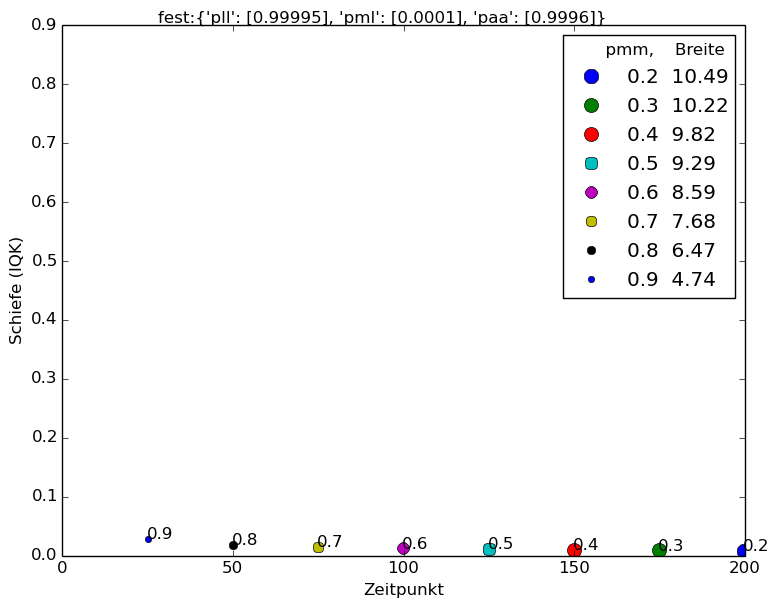
\includegraphics[width=0.49\textwidth]{bilder/pmm/3fest_p_00001_09996_099995}
\caption[Der Einfluss von $p_{mm}$ auf die Peaks abhängig von $p_{aa}$]{Der Einfluss von $p_{mm}$ auf die Peaks abhängig von $p_{aa}$, welches von oben links nach unten rechts größer wird}
\label{einfluss_pmm_1}
\end{figure}

Wie in Abbildung \ref{einfluss_pmm_1} zu sehen, ist der Einfluss von $p_{mm}$ auf den Zeitpunkt von $p_{aa}$ abhängig: Je größer $p_{aa}$ ist, desto stärker wird der Zeitpunkt von $p_{mm}$ beeinflusst. Wenn $p_{mm}$ und $p_{aa}$ klein sind, entstehen nur Peaks zu Beginn des Spektrums, unabhängig von $p_{ml}$ oder $p_{ll}$.

Der Einfluss von $p_{mm}$ auf die Breite ebenfalls von $p_{aa}$ abhängig. Bei größerem $p_{aa}$ steigt dieser Einfluss etwas, wie ebenfalls in Abbildung \ref{einfluss_pmm_1} zu erkennen ist. Dieser Zusammenhang ergibt sich daraus, dass sich in diesem Fall auch der Maximalzeitpunkt nach hinten verschiebt und spätere Peaks generell breiter sind, als frühe Peaks.

\todo{Noch mal den kleinen Bereich untersuchen, wo die Schiefe negativ beeinflusst wird. Das ist ein Bereich, in dem die Peaks zwar eher früh, aber dafür fast zu breit sind. Vielleicht hängt das damit zusammen? siehe: $p_{mm}$0.001 0.998 0.99999}

Außer in einem sehr kleinen Parameterbereich, steigt die Schiefe mit steigendem $p_{mm}$. Dieser Einfluss hängt noch von $p_{aa}$ ab, bei kleinem $p_{aa}$ hat $p_{mm}$ einen größeren Einfluss auf die Schiefe.

\begin{figure}
\begin{subfigure}{0.6\textwidth}
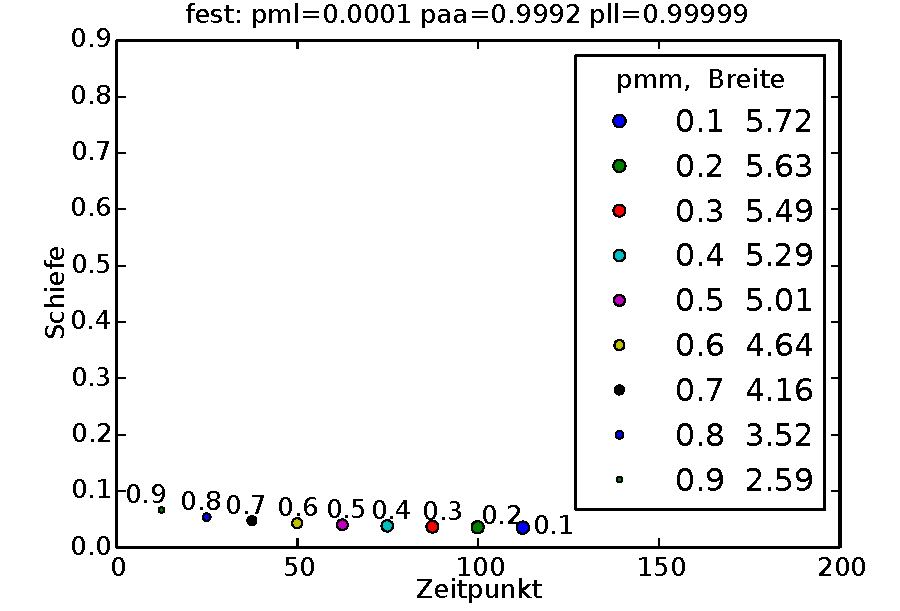
\includegraphics[width=\textwidth]{bilder/pmm/3fest_p_00001_09992_099999}
\caption{$p_{ml}$ klein}
\end{subfigure}

\begin{subfigure}{0.6\textwidth}
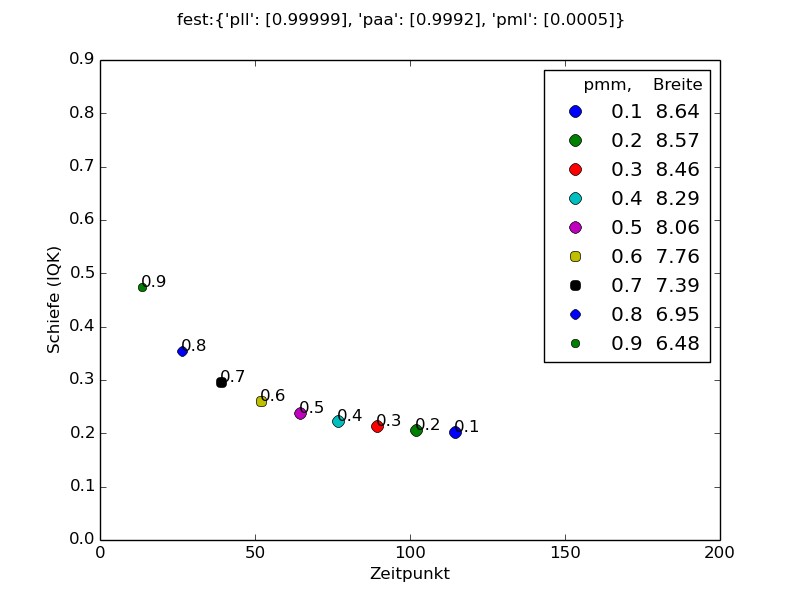
\includegraphics[width=\textwidth]{bilder/pmm/3fest_p_00005_09992_099999}
\caption{$p_{ml}$ mittel}
\end{subfigure}

\begin{subfigure}{0.6\textwidth}
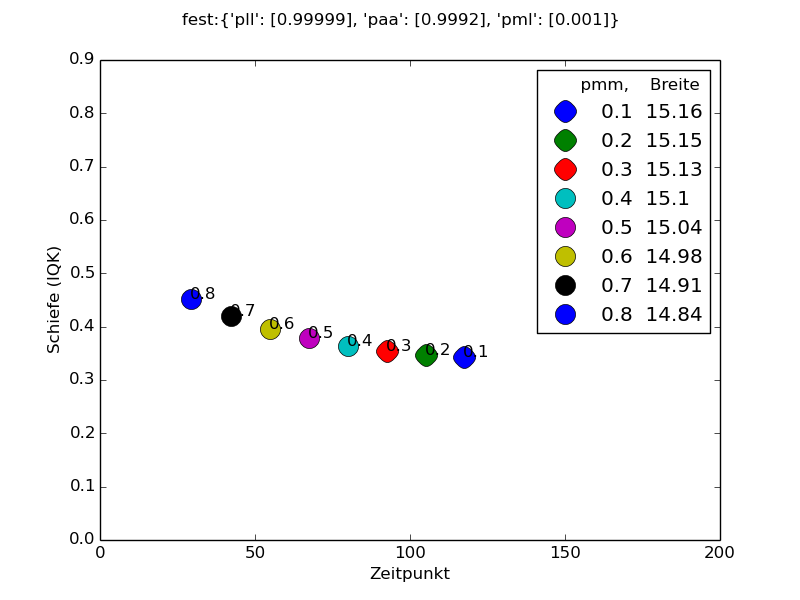
\includegraphics[width=\textwidth]{bilder/pmm/3fest_p_0001_09992_099999}
\caption{$p_{ml}$ groß}
\end{subfigure}
\caption{Der Einfluss von $p_{mm}$ auf die Peaks abhängig von $p_{ml}$}
\label{einfluss_pmm_2}
\end{figure}

Außerdem ist der Einfluss von $p_{mm}$ auf die Schiefe am größten bei mittlerem $p_{ml}$ und (etwa im Intervall $[0,0001, 0,0005]$) und mittlerem $p_{ll}$ (etwa bei $[0,99995; 0,99999]$). Dieser Zusammenhang ist für $p_{ml}$ in Abbildung \ref{einfluss_pmm_2} dargestellt.
Zusätzlich wird der Einfluss von $p_{ml}$ und $p_{ll}$ auf die Abhängigkeit der Schiefe von $p_{mm}$ größer, wenn $p_{aa}$ klein ist.

%Dieser Zusammenhang kann wie folgt erklärt werden. Das Tailing entsteht, wie oben erwähnt, durch seltenes aber sehr langes Verweilen im gelösten Zustand. Bei großem $p_{mm}$ oder kleinem $p_{aa}$ haben die Teilchen die größte Durchschittsgeschwindigkeit, wodurch sie sich im Gesamtverlauf der Säulendurchquerung seltener lösen. Bei langsamerer Durchschittsgeschwindigkeit 

Dieser Zusammenhang kann wie folgt erklärt werden: $p_{ml}$ und $p_{ll}$ verursachen gemeinsam das Tailing. Dieser Effekt kann sich bei großem $p_{mm}$ besser zeigen. Dann sind die Teilchen im Durchschnitt schneller. Ein kleiner Wert für $p_{aa}$ sorgt ebenfalls für eine höhere Durchschnittsgeschwindigkeit. Dadurch geraten im Gesamtverlauf der Säulendurchquerung Teilchen seltener in den gelösten Zustand, wodurch sie das Tailing erzeugen. Bei durchschnittlich langsameren Teilchen lösen sich die Teilchen zu häufig und statt Schiefe entsteht wiederum Breite.
Ist $p_{aa}$ jedoch zu klein und $p_{ll}$ zu groß entstehen Peaks, die einen extrem großen Quartilskoeffizienten haben. %Allerdings ist der Tail so flach, dass er in einem Gesamtchromatogramm wohl eher im Rauschen untergehen würde.

% TODO: Gehört ans Ende: Ist $p_{ml}$ zu klein, hat der gelöste Zustand fast keinen Einfluss und es entsteht unabhängig von $p_{mm}$ kaum Schiefe. Gleiches gilt für $p_{ll}$, ist es zu klein, verweilen die Teilchen nicht lange genug, um Tailing zu verursachen.
% Wenn $p_{ml}$ und $p_{ll}$ jedoch zu groß werden, 
%  ist $p_{ml}$ zu groß, werden die Peaks wieder nur breit, aber nicht so schiefa die Teilchen, die nicht in den gelösten Zustand kommen, sich recht schnell fortbewegen (daher auch besonders bei kleinem $p_{aa}$ zu beobachten) und dadurch nur wenige Teilchen langsamer sind und dadurch den Tail verursachen. Ist $p_{aa}$ kleiner, lösen sich die Teilchen häufiger und statt der schiefen entstehen breite Peaks.


\paragraph*{Einfluss des Parameters $p_{ml}$}

\begin{figure}
\begin{subfigure}[t]{0.49\textwidth}
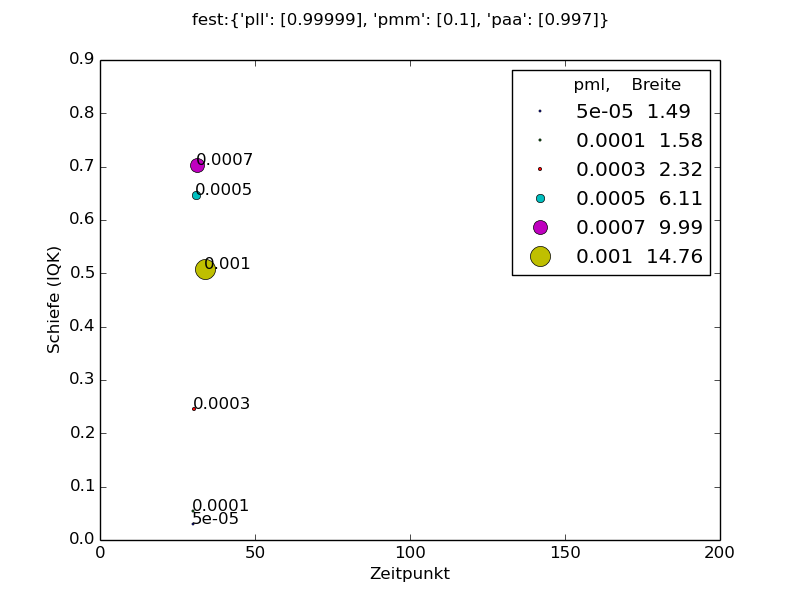
\includegraphics[width=\textwidth]{bilder/pml/pml_01_p_0997_099999}
\caption{$p_{ll}$ sehr groß}
\label{einfluss_pml_pll++}
\end{subfigure}
\begin{subfigure}[t]{0.49\textwidth}
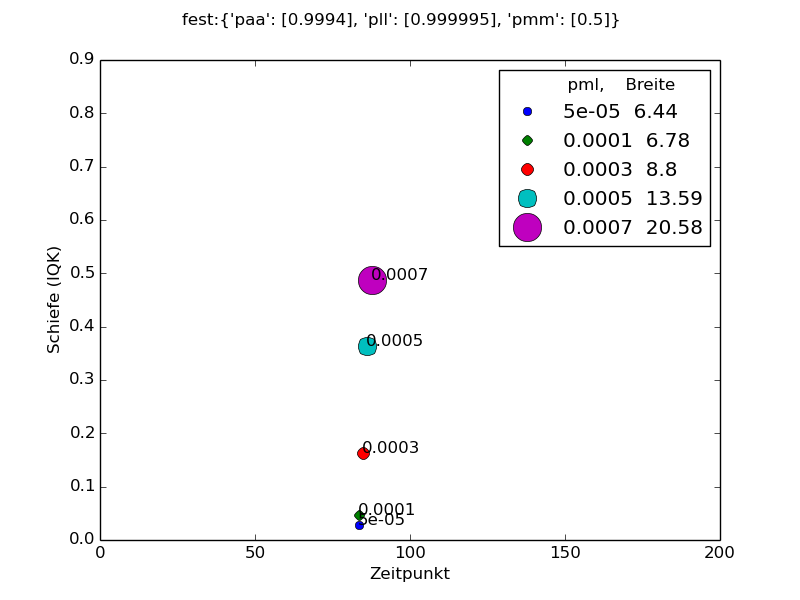
\includegraphics[width=\textwidth]{bilder/pml/pml_05_p_09994_0999995}
\caption{$p_{ll}$ groß}
\label{einfluss_pml_pll+}
\end{subfigure}
\vspace*{7mm}
\begin{subfigure}[b]{0.49\textwidth}
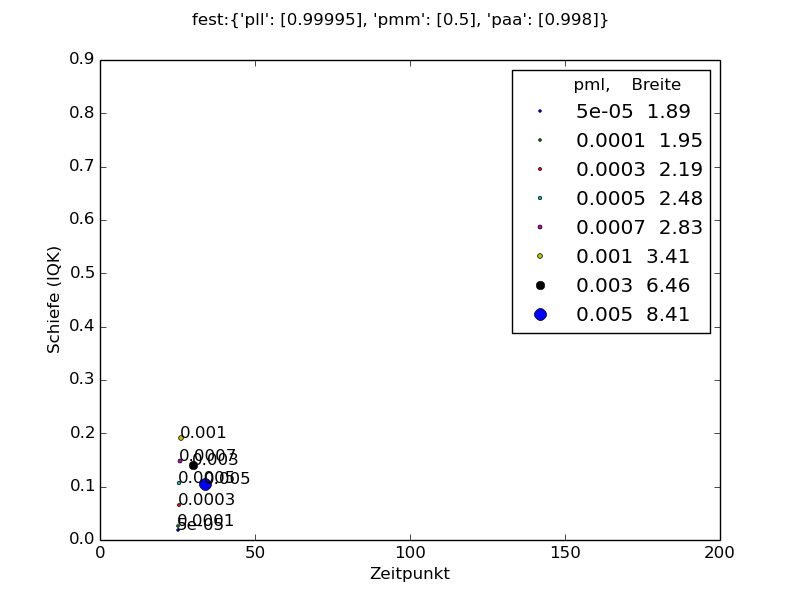
\includegraphics[width=\textwidth]{bilder/pml/pml_05_p_0998_099995}
\caption{$p_{ll}$ klein}
\label{einfluss_pml_pll-}
\end{subfigure}
\begin{subfigure}[b]{0.49\textwidth}
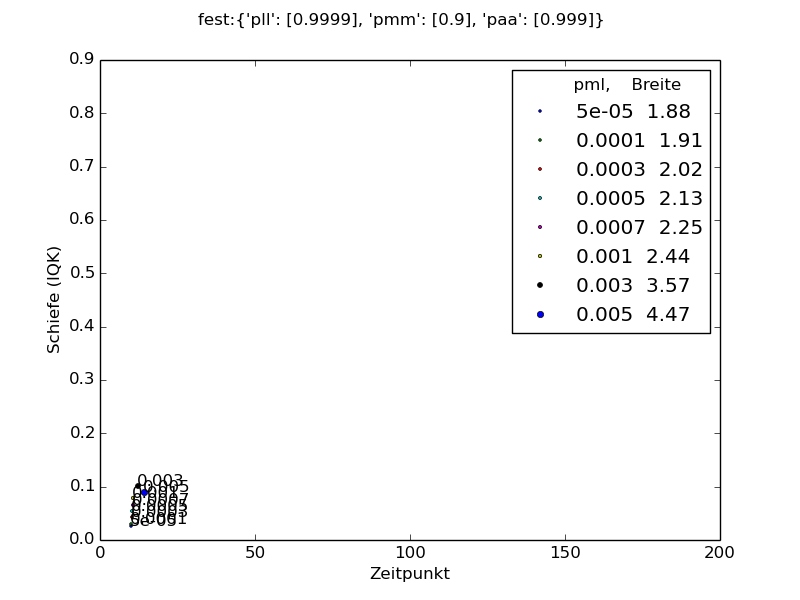
\includegraphics[width=\textwidth]{bilder/pml/pml_09_p_0999_09999}
\caption{$p_{ll}$ sehr klein}
\label{einfluss_pml_pll--}
\end{subfigure}
\caption{Der Einfluss von $p_{ml}$ auf die Schiefe und Breite abhängig von $p_{ll}$}
\label{einfluss_pml_1}
\end{figure}

Der Einfluss von $p_{ml}$ auf die Peakdaten ist in den Abbildungen \ref{einfluss_pml_1} und \ref{einfluss_pml_2} gezeigt. Schiefe und Breite sind häufig deutlich von $p_{ml}$ beeinflusst, der Zeitpunkt hingegen kaum. Allenfalls sehr große Werte für $p_{ml}$ sorgen für einen erkennbar höheren Zeitpunkt, dann aber auch für deutlich mehr Breite und weniger Schiefe.

\begin{figure}
\begin{subfigure}[t]{0.49\textwidth}
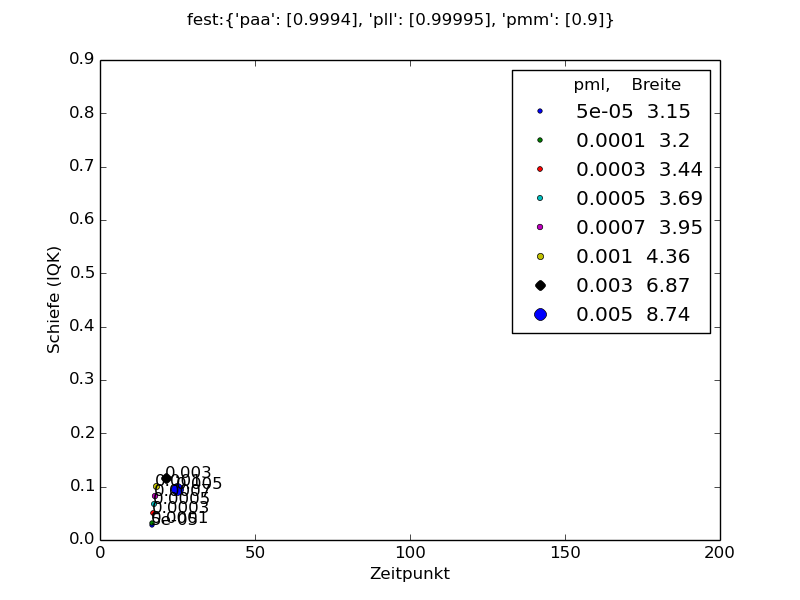
\includegraphics[width=\textwidth]{bilder/pml/pml_09_p_09994_099995}
\caption{$p_{mm}$ groß, $p_{aa}$ groß}
\end{subfigure}
\begin{subfigure}[t]{0.49\textwidth}
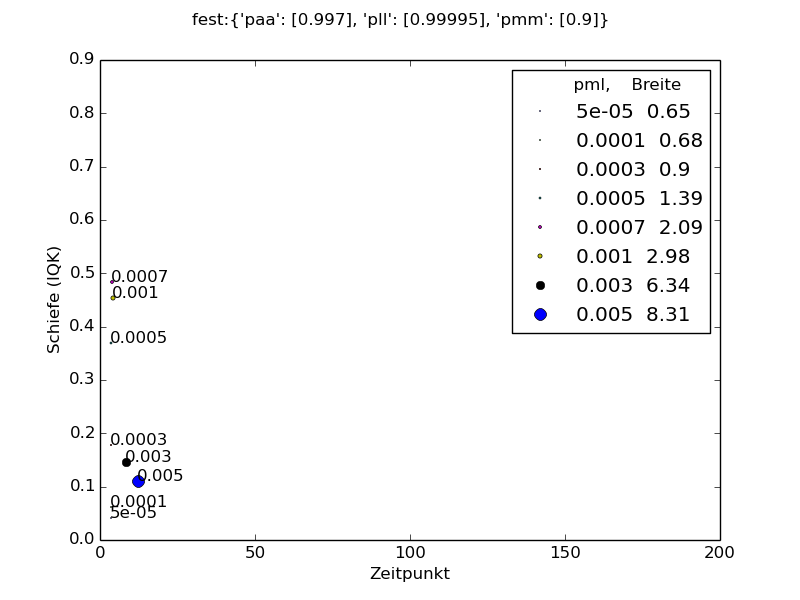
\includegraphics[width=\textwidth]{bilder/pml/pml_09_p_0997_099995}
\caption{$p_{mm}$ groß, $p_{aa}$ klein}
\end{subfigure}
\vspace*{7mm}
\begin{subfigure}[b]{0.49\textwidth}
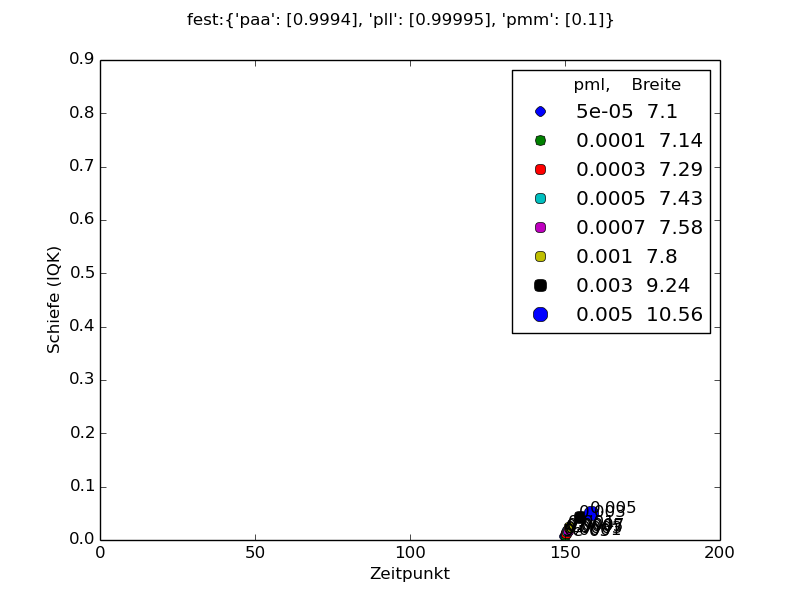
\includegraphics[width=\textwidth]{bilder/pml/pml_01_p_09994_099995}
\caption{$p_{mm}$ klein, $p_{aa}$ groß}
\end{subfigure}
\begin{subfigure}[b]{0.49\textwidth}
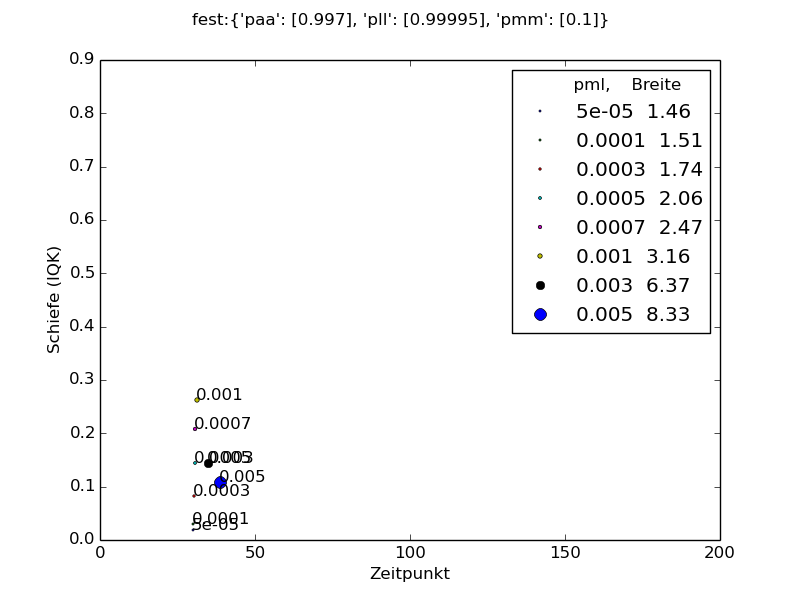
\includegraphics[width=\textwidth]{bilder/pml/pml_01_p_0997_099995}
\caption{$p_{mm}$ klein, $p_{aa}$ klein}
\end{subfigure}
\caption{Der Einfluss von $p_{ml}$ auf die Schiefe und Breite abhängig von $p_{mm}$ und $p_{aa}$}
\label{einfluss_pml_2}
\end{figure}

Auf die Schiefe und Breite ist der Einfluss von $p_{ml}$ sehr groß, wenn auch $p_{ll}$ groß ist, wie in Abbildung \ref{einfluss_pml_1} zu erkennen. Hier sind $p_{mm}$ und $p_{aa}$ auf allen vier Plots gleich gewählt, nur $p_{ll}$ nimmt von \ref{einfluss_pml_pll++} nach \ref{einfluss_pml_pll--} ab und damit schwindet auch der Einfluss von $p_{ml}$ auf Schiefe und Breite.

Wie in Abbildung \ref{einfluss_pml_2} gezeigt, spielen auch $p_{mm}$ und $p_{aa}$ für den Einfluss von $p_{ml}$ auf Schiefe und Breite eine Rolle. Hier ist $p_{ll}$ in allen vier Plots konstant, $p_{mm}$ und $p_{aa}$ werden variiert. Zu erkennen ist, dass bei kleinem $p_{aa}$, der Einfluss von $p_{ml}$ auf Schiefe und Breite größer wird, ist $p_{mm}$ jedoch klein, wird auch der Einfluss von $p_{ml}$ kleiner.


\paragraph*{Einfluss des Parameters $p_{aa}$}

\begin{figure}
% \begin{subfigure}[t]{0.49\textwidth}
% 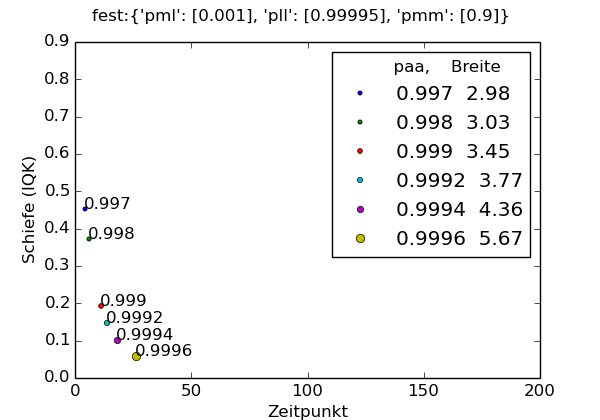
\includegraphics[width=\textwidth]{bilder/paa/3fest_09_0001_p_099995}
% \caption{$p_{mm}$ und $p_{ml}$ groß}
% \end{subfigure}
\begin{subfigure}[t]{0.49\textwidth}
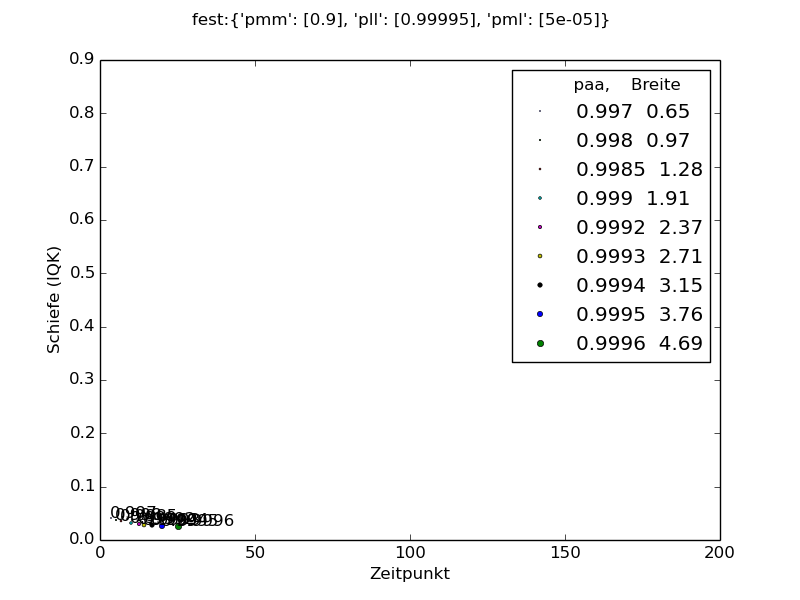
\includegraphics[width=\textwidth]{bilder/paa/3fest_09_5e-05_p_099995}
\caption{$p_{mm}$ groß und $p_{ml}$ klein}
\end{subfigure}
%\vspace*{7mm}
% \begin{subfigure}[b]{0.49\textwidth}
% 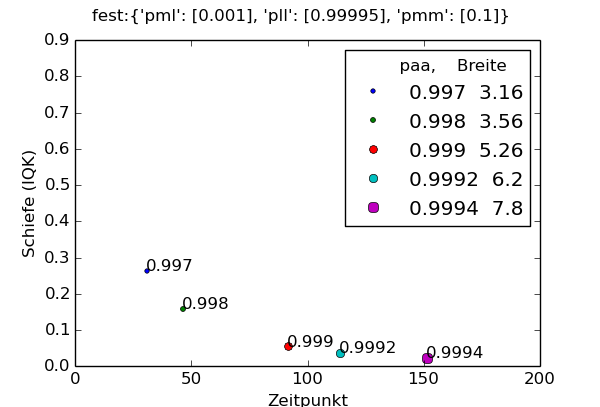
\includegraphics[width=\textwidth]{bilder/paa/3fest_01_0001_p_099995}
% \caption{$p_{mm}$ klein und $p_{ml}$ groß}
% \end{subfigure}
\begin{subfigure}[t]{0.49\textwidth}
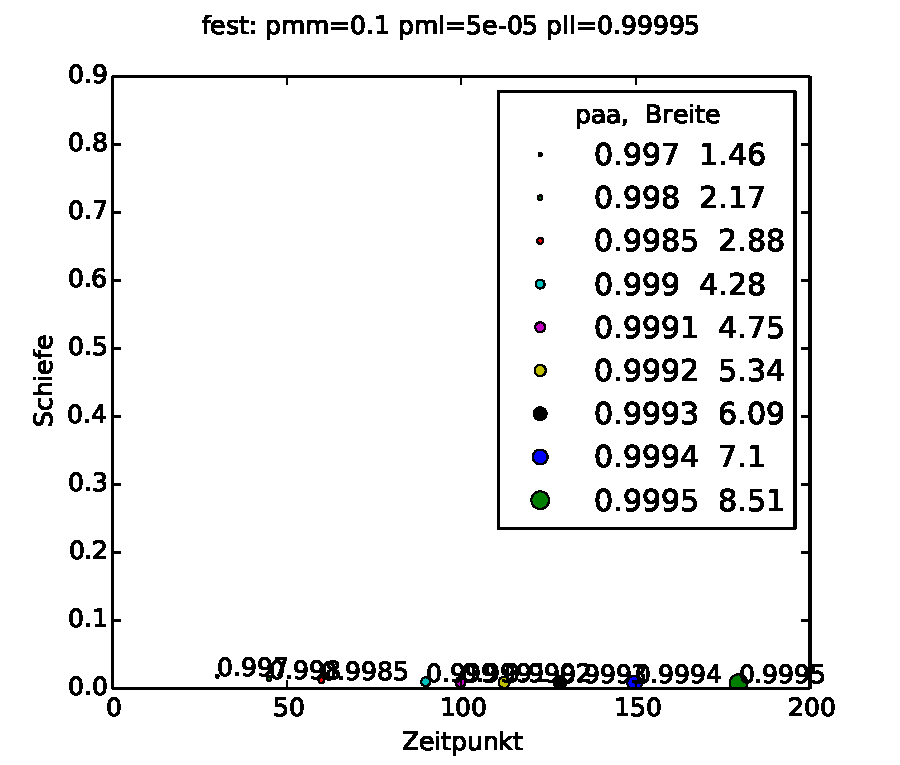
\includegraphics[width=\textwidth]{bilder/paa/3fest_01_5e-05_p_099995}
\caption{$p_{mm}$ und $p_{ml}$ klein}
\end{subfigure}
\caption{Der Einfluss von $p_{aa}$ auf die Peaks abhängig von $p_{mm}$}
\label{einfluss_paa}
\end{figure}

In Abbildung \ref{einfluss_paa} ist beispielhaft der Einfluss von Parameter $p_{aa}$ in Abhängigkeit von $p_{mm}$ auf die Peaks gezeigt. Der Einfluss von $p_{aa}$ auf den Zeitpunkt wird mit steigendem $p_{mm}$ immer kleiner und reicht dadurch von minimalem Einfluss und recht frühen Peaks bei jeder Wahl von $p_{aa}$ bis zu sehr großem Einfluss und Peaks, die je nach $p_{aa}$ über das ganze Spektrum verteilt sind. Damit hat $p_{aa}$ einen ähnlichen Einfluss wie $p_{mm}$.

\begin{figure}
\begin{subfigure}{0.6\textwidth}
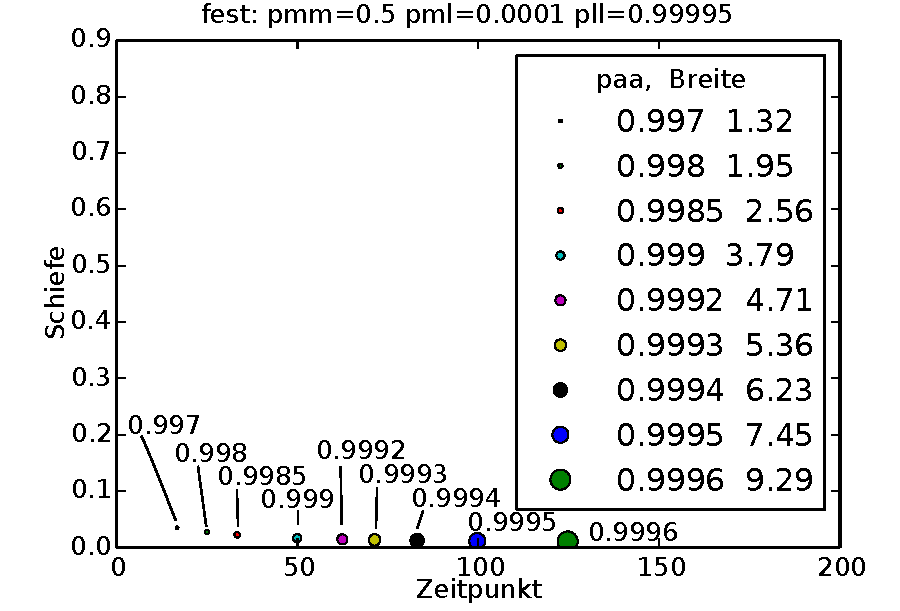
\includegraphics[width=\textwidth]{bilder/paa/3fest_05_00001_p_099995}
\caption{$p_{ml}$ klein}
\end{subfigure}

\begin{subfigure}{0.6\textwidth}
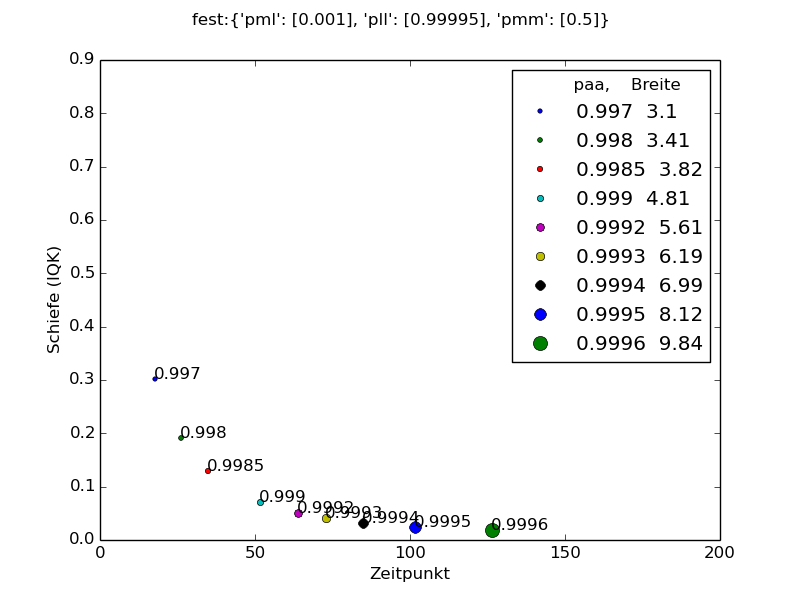
\includegraphics[width=\textwidth]{bilder/paa/3fest_05_0001_p_099995}
\caption{$p_{ml}$ mittel}
\end{subfigure}

\begin{subfigure}{0.6\textwidth}
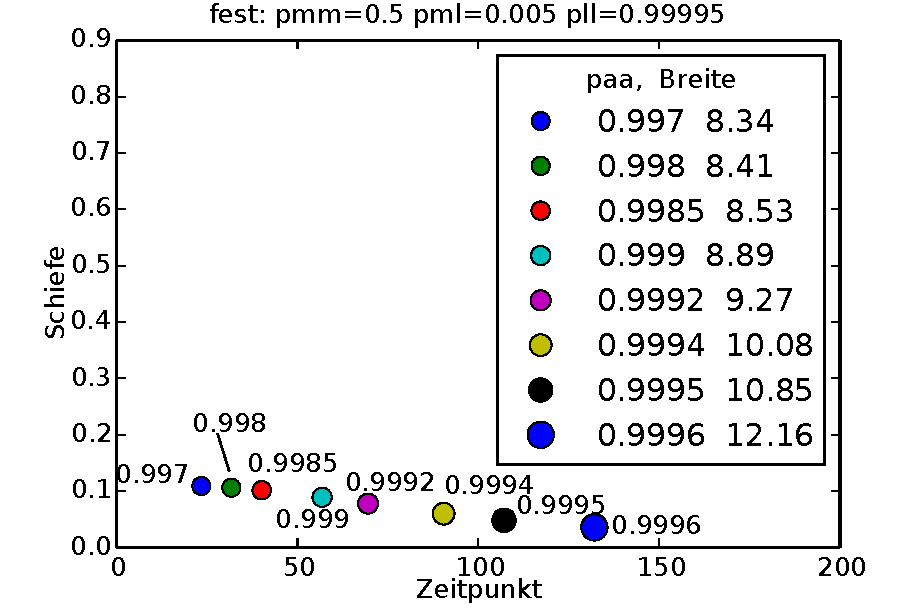
\includegraphics[width=\textwidth]{bilder/paa/3fest_05_0005_p_099995}
\caption{$p_{ml}$ groß}
\end{subfigure}
\caption{Der Einfluss von $p_{aa}$ auf die Peaks abhängig von $p_{ml}$}
\label{einfluss_paa_pml}
\end{figure}

Wie in \ref{einfluss_paa_pml} zu sehen $p_{aa}$ hat nur dann einen relevanten Einfluss auf die Schiefe, wenn $p_{ml}$ mittelgroß ist (um $0,0007$ herum). Bei zu großem $p_{ml}$ werden Peaks statt dessen wieder nur breit und bei zu kleinem $p_{ml}$ hat $p_{aa}$ kaum Einfluss auf die Schiefe. 

Der Einfluss auf die Breite ist mäßig und wird größer, wenn $p_{ml}$ und $p_{ll}$ klein sind, für $p_{ml}$ ist dies ebenfalls in Abbildung \ref{einfluss_paa_pml} zu erkennen.

TODO: $p_{ll}$ verändert auch den Einfluss von $p_{aa}$, das hängt aber von $p_{mm}$ und $p_{ml}$ ab und sämtlichen konkreten Werten ab.

\paragraph*{Einfluss des Parameters $p_{ll}$}

Der Einfluss von $p_{ll}$ auf den Zeitpunkt ist ähnlich wie bei $p_{ml}$ nur minimal.

\begin{figure}
\begin{subfigure}[t]{0.49\textwidth}
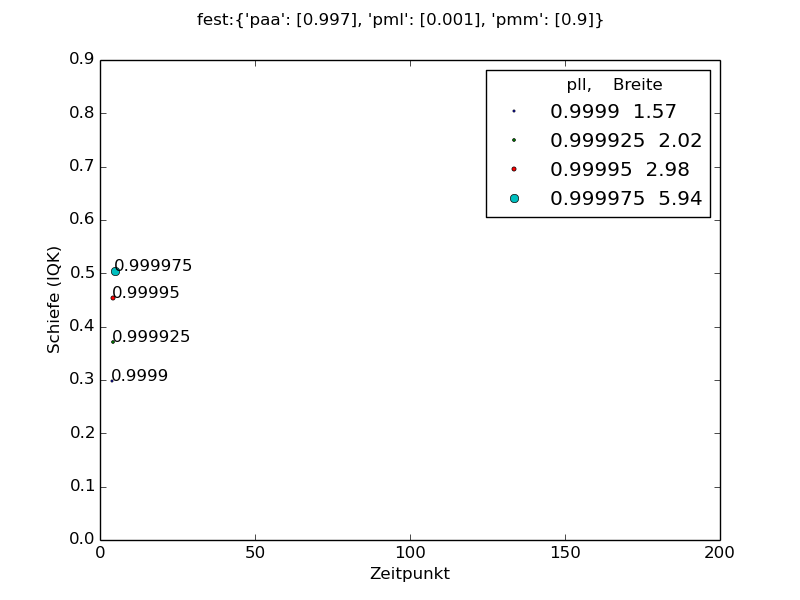
\includegraphics[width=\textwidth]{bilder/pll/3fest_09_0001_0997_p}
\caption{$p_{ml}$ sehr groß}
\label{einfluss_pll_pml++}
\end{subfigure}
\begin{subfigure}[t]{0.49\textwidth}
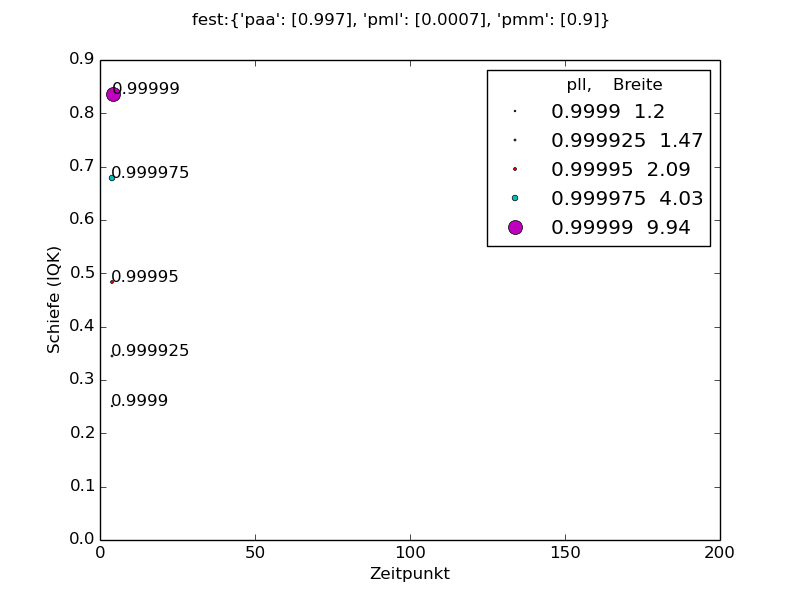
\includegraphics[width=\textwidth]{bilder/pll/3fest_09_00007_0997_p}
\caption{$p_{ml}$ groß}
\label{einfluss_pll_pml+}
\end{subfigure}
\vspace*{7mm}
\begin{subfigure}[b]{0.49\textwidth}
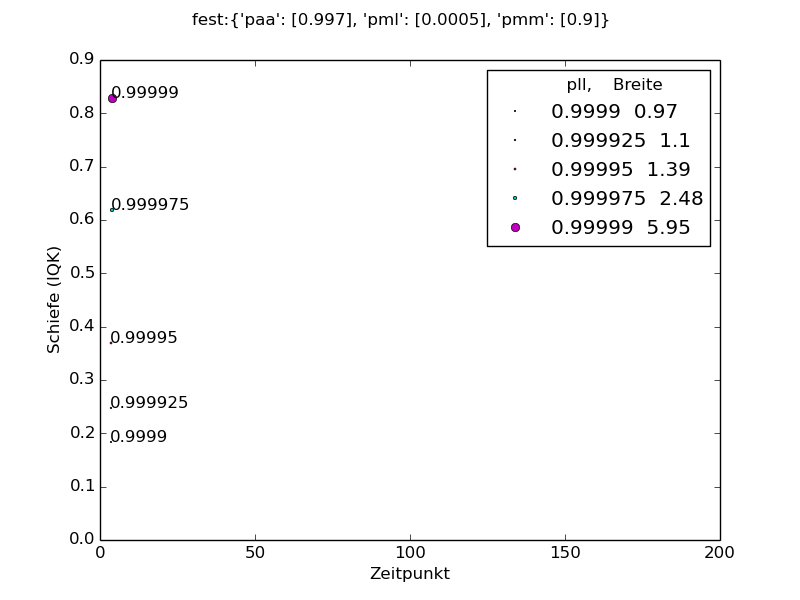
\includegraphics[width=\textwidth]{bilder/pll/3fest_09_00005_0997_p}
\caption{$p_{ml}$ klein}
\label{einfluss_pll_pml-}
\end{subfigure}
\begin{subfigure}[b]{0.49\textwidth}
\includegraphics[width=\textwidth]{bilder/pll/3fest_09_00003_0997_p}
\caption{$p_{ml}$ sehr klein}
\label{einfluss_pll_pml--}
\end{subfigure}
\caption{Der Einfluss von $p_{ll}$ auf die Schiefe und Breite abhängig von $p_{ml}$}
\label{einfluss_pll_pml}
\end{figure}

Auf Breite und Schiefe hat $p_{ll}$ einen von $p_{ml}$ abhängigen Einfluss: Wenn $p_{ml}$ mittelgroß ist, ist die Wirkung von $p_{ll}$ am größten. Das ist in Abbildung \ref{einfluss_pll_pml} gezeigt.

\begin{figure}
\begin{subfigure}[b]{0.49\textwidth}
\includegraphics[width=\textwidth]{bilder/pll/3fest_01_00005_0999_p}
\caption{$p_{mm}$ klein}
\end{subfigure}
\begin{subfigure}[b]{0.49\textwidth}
\includegraphics[width=\textwidth]{bilder/pll/3fest_09_00005_0999_p}
\caption{$p_{mm}$ groß}
\end{subfigure}
\caption{Der Einfluss von $p_{ll}$ auf die Peaks abhängig von $p_{mm}$}
\label{einfluss_pll_pmm}
\end{figure}

\begin{figure}
\begin{subfigure}[b]{0.49\textwidth}
\includegraphics[width=\textwidth]{bilder/pll/3fest_03_00003_0998_p}
\caption{$p_{aa}$ klein}
\end{subfigure}
\begin{subfigure}[b]{0.49\textwidth}
\includegraphics[width=\textwidth]{bilder/pll/3fest_03_00003_09994_p}
\caption{$p_{aa}$ groß}
\end{subfigure}
\caption{Der Einfluss von $p_{ll}$ auf die Peaks abhängig von $p_{aa}$}
\label{einfluss_pll_paa}
\end{figure}

Wenn $p_{ml}$ nicht zu klein oder groß ist, hat $p_{ll}$ einen großen Einfluss auf Schiefe und Breite. Dieser Einfluss wächst, je größer $p_{mm}$ und je kleiner $p_{aa}$ ist. Dies ist in \ref{einfluss_pll_pmm} für $p_{mm}$ und in \ref{einfluss_pll_paa} für $p_{aa}$ zu sehen. 
%(Hängt wieder mit der Durchschnittsgeschwindigkeit zusammen)


Zusammengefasst: 
\todo{Noch mal ganz kurz zusammenfassen, welche Peakmerkmale wodurch maßgeblich bestimmt werden}
TODO: Das folgende ist zwar interssant, aber eher so eine Zusammenfassung
Da bei einem Wert von $0$ für $p_{ml}$ effektiv das 2-Zustände Modell zum Einsatz kommt, ist hier fast nie Schiefe zu beobachten, außerdem hat der Parameter $p_{ll}$ keinen Einfluss. 

$p_{aa}$ hat einen stärkeren Einfluss auf den Zeitpunkt als $p_{ll}$ und $p_{ml}$. Dieser wird noch stärker, wenn $p_{mm}$ klein ist

$p_{mm}$ hat einen großen Einfluss auf den Zeitpunkt und nur einen minimalen Einfluss auf die Breite.

$p_{ml}$ und $p_{ll}$ haben zunächst beide einen proportionalen Einfluss auf die Schiefe. Erst, wenn beide sehr groß sind, sinkt die Schiefe wieder (und die Breite steigt extrem an) Das ist wohl dadurch zu erklären, dass sich nicht mehr genügend Teilchen im mobil-adsorbierten System befinden, wodurch ein normaler Peak entstehen kann. Statt dass die Lösung Schiefe an diesem einfachen Peak verursacht, sorgt sie nunmehr für Breite

Tailing/Schiefe entsteht immer da, wo nur wenige Teilchen langsamer sind, als die große Masse. Sind viele Teilchen lange stationär, werden die Peaks statt dessen breit. Der Maximalzeitpunkt ist hauptsächlich durch die Durchschnittsgeschwindigkeit der Teilchen bestimmt, sind sie hauptsächlich mobil, entstehen frühe Peaks, sind sie oft und lange stationär, wandern die Peaks nach hinten.


\subsubsection{Parameter für ähnliche Peaks}

Durch die vielfältigen und unterschiedlich starken Einflüsse der einzelnen Parameter, ist es möglich, fast gleiche Peaks mit völlig unterschiedlichen Parameterkombinationen zu erzeugen. Zwei Beispiele dafür sind in den Abbildungen \ref{2kombis_1} und \ref{2kombis_2} gezeigt.

\begin{figure}[h]
\includegraphics[width=0.49\textwidth]{bilder/kombis/1peak1_kombi1}
\includegraphics[width=0.49\textwidth]{bilder/kombis/1peak1_kombi2}
\caption{Sehr ähnliche Peaks bei $t \approx 25$}
\label{2kombis_1}
\end{figure}

\begin{figure}[h]
\includegraphics[width=0.49\textwidth]{bilder/kombis/1peak2_kombi1}
\includegraphics[width=0.49\textwidth]{bilder/kombis/1peak2_kombi2}
\caption{Sehr ähnliche Peaks bei $t \approx 100$}
\label{2kombis_2}
\end{figure}

\todo{Achsenbeschrifung}

In beiden Fällen unterscheiden sich die resultierenden Peaks kaum, sie könnten jedoch durch minimale Parameterveränderungen noch stärker angenähert werden. Die Zuordnung von Simulationsparameter zu Peakcharakteristika ist also nicht eindeutig.

\section{Grenzen des Modells}

Mit dem 2-Zustände Modell war es nur eingeschränkt möglich, Tailing zu erzeugen. Insbesondere tritt kein Tailing nicht zu den späteren Zeitpunkten im Chromatogramm auf. Diese Einschränkung konnte, wie gezeigt wurde, mit dem 3-Zustände Modell aufgehoben werden. 

Das andere Problem jedoch, dass Peaks zu jedem Zeitpunkt eine Minimalbreite haben, konnte dadurch jedoch nicht gelöst werden. Die Peaks können durch Hinzunahme eines weiteren stationären Zustandes höchstens breiter werden. 

\section{Laufzeiten}
\todo{Wohin mit Laufzeiten? Hier und Implementierung!}

 